\documentclass[10pt, openright,oneside]{book}
\usepackage[a4paper,width=150mm,top=25mm,bottom=25mm]{geometry}
\usepackage{csquotes} %fixes some error

\usepackage[english]{babel}
\usepackage{subfiles}
\usepackage{float} % keepd tables etc in place
\usepackage{wrapfig}

% Removes paragraph indentation (not needed most of the time now)
\usepackage{parskip}

% Provides ways to make nice looking tables
\usepackage{booktabs}
% Typesets URLs sensibly - with tt font, clickable in PDFs, and not breaking across lines
\usepackage{url}
\usepackage{hyperref}
\hypersetup{
    colorlinks=true,
    linkcolor=black,
    citecolor=gray,
    filecolor=magenta,      
    urlcolor=cyan,
}
 
\usepackage{mwe}% for putting 2 images side by side
\usepackage[font={footnotesize},labelfont=bf]{caption}

\usepackage[usenames, dvipsnames]{color} %text color

\usepackage[table,xcdraw]{xcolor}
\usepackage{multirow}

%abbreviations management 
\usepackage{nomencl}
\makenomenclature
\renewcommand*{\nompreamble}{\small}
\renewcommand{\nomname}{List of Abbreviations}

% for adding pretty headings
%\usepackage{fancyhdr}
%\pagestyle{fancy}

\usepackage[utf8]{inputenc}
\usepackage{graphicx}
\graphicspath{ {images/} }
\usepackage{wallpaper}

\usepackage[backend=biber,style=ieee]{biblatex}
\addbibresource{mendeley.bib}
\addbibresource{nonmenrefs.bib}

%allows subsub sections and paragraphs
\setcounter{tocdepth}{4}
\setcounter{secnumdepth}{4}

%\usepackage{refcount} %for making lists of fig appear in contents
\usepackage[nottoc]{tocbibind}
\begin{document}


\frontmatter
%%  Begin title page
%%  ==================================================================
    \thispagestyle{empty}
    \ULCornerWallPaper{1}{ku-coverpage/nat-farve.pdf}
    \ULCornerWallPaper{1}{ku-coverpage/nat-en.pdf}
    %\begin{adjustwidth}{-1cm}{-0.5cm}
    
    \vspace*{4.5cm} 
    \noindent \textbf{\huge Identification of autophagy signatures\\ in breast cancer using\\ The Cancer Genome Atlas data} \\
    \\[0.5cm]
    \textit{\Large Master's Thesis} \\
    [0.5cm]
    \textbf{\Large MSc Bioinformatics} \\
    \vspace*{.1cm} \\
%     {\huge Subtitle} \\
    \begin{tabbing}
    % adjust the hspace below for the longest author name
    \textbf{Marina Vabistsevits} \hspace{1cm} \= \texttt{<rzq995@alumni.ku.dk>} \\
    \\[9cm]
    \textbf{\Large Supervisors} \\
    Dr Elena Papaleo \> \texttt{<elenap@cancer.dk>} \\
    Prof Albin Sandelin \> \texttt{<albin@binf.ku.dk>} \\
    Dr Kristoffer Vitting-Seerup\> \texttt{<kristoffer.vittingseerup@bio.ku.dk>}
    \\[1cm]
    
    \end{tabbing}
    \begin{center}
    \textit{7 August, 2017} 
    \end{center}
    %\end{adjustwidth}

    \newpage
    \ClearWallPaper
    
%%  ==================================================================
%%  End title page



\pagestyle{plain}


\frontmatter

\chapter{Abstract}
Breast cancer is the second leading cause of death among women in developed countries. It is an extremely heterogeneous disease with distinct subtypes and clinical implications. One of the mechanisms through which cancer development could be controlled is autophagy. Autophagy is a highly-conserved process of cellular self-degradation in response to stress or nutrient starvation. It can promote both cell-survival and cell-death, hence it has been linked to many human pathologies including cancer. In cancer, autophagy is believed to have a complex and context-dependent role. At initial stages of cancer, it helps to recycle damaged molecules thereby reducing cytotoxic damage and preventing tumorogenesis. Impaired autophagy contributes to cancer progression. At later stages of cancer, tumour cells learn to use autophagy for their own cytoprotection and thereby evade cancer therapies. 

However, the current understanding of the exact link between autophagy regulation and breast cancer development is very superficial and there are many unanswered questions. Both breast cancer and autophagy research fields have seen a number of highlights and breakthroughs in the past decade, therefore now it is time to start bridging the knowledge gap between the two by identifying autophagy signatures in breast cancer. 

In this project, data from one of the largest publicly available cancer resources, The Cancer Genome Atlas, was used to analyse gene expression changes between various breast cancer classification subgroups, including tumour morphology, cancer stage, and PAM50 molecular profile. The sample classification subgroups were extensively investigated with different exploratory analysis methods, which confirmed the tremendous heterogeneity of breast cancer. The exploratory analysis results were used to guide the differential expression analysis setup. Additionally, soft-clustering was performed to detect clusters of genes that have similar expression behaviour with respect to their changes along cancer stages. Following that, differentially expressed genes and the genes assigned to individual clusters were tested for autophagy enrichment. 

The enrichment analysis has shown that autophagy genes are overrepresented among the genes that are downregulated in cancer versus normal, regardless of subtype or morphology. This signature was found both in differential expression analysis and soft-clustering results. A consensus set of genes between the results of two methods was identified, thereby providing a list of candidate autophagy genes that can be further explored for their role in breast cancer. 



\tableofcontents

\cleardoublepage
\addcontentsline{toc}{part}{\small List of Abbreviations}
\addtocontents{toc}{\protect\vspace{-0.1em}}
%abbreveations
\printnomenclature[6em]
\hfill % add blank space

\nomenclature{AJCC}{The American Joint Committee on Cancer }
\nomenclature{CBL}{Computational Biology Lab}
\nomenclature{CPM}{Counts per million}
\nomenclature{DCRC}{Danish Cancer Research Centre}
\nomenclature{DE}{Differential expression / differentially expressed }
\nomenclature{DEA}{Differential expression analysis }
\nomenclature{DEGs}{Differentially expressed genes }
\nomenclature{EDA}{Exploratory data analysis}
\nomenclature{ER}{Estrogen receptor}
\nomenclature{GDC}{Genomic Data Commons }
\nomenclature{HER2}{Human epidermal growth factor receptor 2 }
\nomenclature{ICD-O-3}{International Classification of Diseases for Oncology, 3rd edition}
\nomenclature{IDC}{Invasive ductal carcinoma }
\nomenclature{IHC}{Immunohistochemistry}
\nomenclature{ILC}{Invasive lobular carcinoma}
\nomenclature{NCI}{National Cancer Institute }
\nomenclature{NHGRI}{National Human Genome Research Institute}
\nomenclature{PCA}{Principal component analysis }
\nomenclature{PCs}{Principal components}
\nomenclature{PR}{Progesterone receptor}
\nomenclature{RPKM}{Reads per kilobase of transcript per million}
\nomenclature{FPKM}{Fragments per kilobase of transcript per million}
\nomenclature{TCGA}{The Cancer Genome Atlas}
\nomenclature{TCGA-BRCA}{The Cancer Genome Atlas breast cancer data}
\nomenclature{TNM}{Tumour, Nodes, Metastasis (system)}
\nomenclature{UICC}{International Union Against Cancer }
\nomenclature{WHO}{World Health Organisation }
\nomenclature{TNBC}{Triple Negative Breast Cancer }
\nomenclature{qRT-PCR}{Quantitative reverse transcriptase polymerase chain reaction }
\nomenclature{PAM50}{Prediction Analysis of Microarray, based on 50 gene set}
\nomenclature{DCC}{Data Coordinating Centre}
\nomenclature{PAS}{Phagophore assembly site}
\nomenclature{PE}{Phosphatidylethanolamine}
\nomenclature{ATG}{Autophagy-related gene}
\nomenclature{PI3P}{Phosphatidylinositol 3-phosphate}
\nomenclature{LIR}{LC3-interacting region}
\nomenclature{ROS}{Reactive oxygen species}

\listoffigures
\listoftables

\mainmatter


\chapter{Introduction}



\section{Scientific background}

    \subsection{Breast Cancer Overview}
   
    Breast cancer is the leading cause of cancer-related deaths among women in developed countries \cite{ferlay2015cancer}. It has been estimated that approximately 2.4 million females developed breast cancer in 2015, and it was the cause of death for more than 520,000 individuals \cite{Fitzmaurice2017Global2015}.  Denmark has the second highest disease incidence rate per 100,000 individuals in the world \cite{2015BreastInternational}. 
    
    Screening programs, education, and improved therapeutic strategies have decreased the mortality rates from this disease, but not at the desired magnitude. The most plausible explanation for this discordance is the lack of a complete picture of the biologic heterogeneity of breast cancers \cite{Vidal2017}.
    Breast cancer is not a single disease, but is composed of multiple subtypes with distinct morphologies and clinical implications \cite{Dai2015}. Growing evidence implies that carcinomas with different histopathological and biological features exhibit distinct behaviours that lead to different treatment responses and require tailored therapeutic approaches \cite{Blows2010}. Therefore, accurate grouping of breast cancers into clinically relevant subtypes is of high importance for prognosis prediction and treatment decision making.

    \subsection{Disease Management and Prognosis}
    
    Historically, prognostication in breast cancer has relied on the clinicopathological parameters such as patient age, tumour size, lymph node involvement, presence of metastasis, histological grade, and individual molecular markers such as hormone receptors, human epidermal growth factor status (HER2), and proliferation marker Ki67. All of these are routinely used in clinics to stratify patients for prognostic predictions, to assign treatments, and to include patients into clinical trials \cite{Vidal2017}.

    The limitations of these markers in predicting risk of recurrence has led to the use of mRNA- and DNA-based markers. The advent of high-throughput platforms for gene expression profiling has shown that tumour cell response to treatment is not determined by anatomical prognostic factors but rather intrinsic molecular characteristics \cite{Iwamoto2010PredictingData}. The large-scale analysis of the genetic makeup of tumours has permitted understanding of the genomic and transcriptomic landscape of breast cancer. It has brought the concept of breast cancer heterogeneity to the forefront of cancer research, and the fact that distinct subtypes of breast cancer are completely different diseases that affect the same anatomical site \cite{weigelt2010}. This new strategy has changed how breast cancer patients are managed and treated, which provided an incremental increase on the reproducibility and accuracy of disease prognosis and therapy selection \cite{pusztai2008}. Importantly, though, the prognostic and predictive power of molecular profiling has been shown to be complementary to, rather than a replacement for, traditional clinicopathological parameters \cite{weigelt2010}.

   
    \subsection{Classification Conventions}
    
    Breast cancers can be classified by different schemata. Each of these aspects influences treatment response and prognosis.  This section will present the main traditional and novel breast cancer classification conventions to introduce the overwhelming heterogeneity observed among the patients. 
    %[more about heterogeneity?]

    \subsubsection{Cancer Staging by TNM}
    
    Cancer staging is a way of determining and describing cancer location and spread in the body. The underlying purpose of staging is to characterise the extent or severity of an individual’s cancer, and to bring together cancers that have similar prognosis and treatment \cite{2017AJCCStaging}. 

    Breast cancer is staged using the TNM system developed by The American Joint Committee on Cancer (AJCC) and the International Union Against Cancer (UICC) \cite{Giuliano2017}. The TNM staging system is the most common tool used by clinicians to converge the results from diagnostic tests and scans, and it involves two steps. Firstly, cancer is classified by several factors, \textbf{T} for the extent of the tumour, \textbf{N} for the extent of spread to the nodes, and \textbf{M} for the presence of metastasis. Then, these are grouped as TNM factors to find the overall cancer stage. Table \ref{table:tnmstage} shows the overview of TNM combinations. There are 5 stages: stage 0 (zero), which is noninvasive \textit{in situ} carcinoma, and stages I through IV (1 through 4), which are used for invasive breast cancer.


    % TNM TABLE
        \begin{table}[!h]
        \centering
        \tiny
        \caption[Cancer staging/ prognostic groups TNM system reference table (from AJCC/UICC)]{Cancer staging/ prognostic groups TNM system reference table (from AJCC/UICC). The combination of T, N, and M is used to assign the  overall stage (substage).}
        \label{table:tnmstage}
        \begin{tabular}{c|c|c|c|c}
        \multicolumn{2}{c|}{\textbf{\small Stage}} & \textbf{Tumour} & \textbf{Nodes} & \textbf{Metastasis} \\ \hline
        \textbf{0} & 0 & Tis & N0 & M0 \\ \hline
        \textbf{1} & IA & T1 & N0 & M0 \\ \hline
        \textbf{} & IB & T0 & N1mi & M0 \\ \cline{2-5} 
        \textbf{} &  & T1 & N1mi & M0 \\ \hline
        \textbf{2} & IIA & T0 & N1 & M0 \\ \hline
        \textbf{} &  & T1 & N1 & M0 \\ \cline{2-5} 
        \textbf{} &  & T2 & N0 & M0 \\ \cline{2-5} 
        \textbf{} & IIB & T2 & N1 & M0 \\ \cline{2-5} 
        \textbf{} &  & T3 & N0 & M0 \\ \hline
        \textbf{3} & IIIA & T0 & N2 & M0 \\ \hline
         &  & T1 & N2 & M0 \\ \cline{2-5} 
         &  & T2 & N2 & M0 \\ \cline{2-5} 
         &  & T3 & N1 & M0 \\ \cline{2-5} 
         &  & T3 & N2 & M0 \\ \cline{2-5} 
         & IIIB & T4 & N0 & M0 \\ \cline{2-5} 
         &  & T4 & N1 & M0 \\ \cline{2-5} 
         &  & T4 & N2 & M0 \\ \cline{2-5} 
         & IIIC & Any T & N3 & M0 \\ \hline
        \textbf{4} & IV & Any T & Any N & M1 \\ \hline
        
        \hline
        \multicolumn{5}{l}{%
          \begin{minipage}{5cm}%
            \tiny M0 includes cM0(i+). N1mi indicates cancer in the axillary lymph nodes  $>0.2mm$ but $<2mm$ (micro-metastasis). \textit{Table is adapted from \cite{Giuliano2017}.} 
          \end{minipage}%
        }\\
        \end{tabular}
        \end{table}


    \textbf{T} – The tumour values (\texttt{TX, T0, Tis, T1, T2, T3 or T4}) depend on the cancer at the primary site of origin in the breast. \texttt{TX} refers to an inability to assess that site; \texttt{T0} means no evidence of primary tumour;  \texttt{Tis} refers to noninvasive \textit{in situ} carcinoma or Paget's disease \cite{Giuliano2017}. The numbered \texttt{T}'s refer to the size of the tumour, ranging from less that 1mm to larger than 50mm in the greatest dimension \cite{2017AJCCStaging}. 

    \textbf{N} – The lymph node values (\texttt{NX, N0, N1, N2 or N3}) depend on the number, size and location of breast cancer cell deposits in various regional lymph nodes, such as the armpit (axillary lymph nodes), the collar area (supraclavicular lymph nodes), and inside the chest (internal mammary lymph nodes) \cite{scatarige1990}. \texttt{N0} refers to no regional node metastases. 
    
    
    \textbf{M} – The two metastatic values (\texttt{M0 and M1}) refer respectively to no clinical or radiographic evidence of distant metastases, and the presence of breast cancer cells in locations other than the breast and regional lymph nodes, such as to bone, brain, lung, i.e. detectable distant metastases. Another recently introduced category between the two, \texttt{cM0(i+)}, refers to molecularly or microscopically detected tumour cells in circulating blood, bone marrow or non-regional nodal tissue, no larger than 0.2 mm, but without evidence or symptoms or signs of metastases \cite{Giuliano2017}, and which, does not change the stage grouping. 
    
    
    Historically, the TNM anatomic stage groups have been associated with outcome measures, including overall survival and disease-free survival \cite{Giuliano2017}.  For groups of patients it provides an accurate prediction of outcome, but within stage groups at individual patient level, outcome predictions are more problematic, as they have different biologic subtypes of cancers that express different biomarkers. In this way, while TNM classification remains the basis for cancer staging, but other factors, such as receptor status, histology, and molecular subtype are now incorporated into parallel prognostic stage groups. Despite the predictive power of intrinsic breast cancer subtypes (e.g. PAM50 classifier, discussed in section X),  the anatomic TNM classification provides a common language for communicating disease burden.

   \subsubsection{Tumour Morphology}
   
   
   Breast cancers are heterogeneous tumours that show a wide variation not only with regard to their clinical presentation and behaviour, but also morphological spectrum. The majority (95\%) of breast tumours are adenocarcinomas -- cancers that arise from the epithelial lining of the breast components \cite{Makki2015DiversityRelevance}, such as ducts and lobules.

    The main division between mammary carcinomas is whether it is \textit{in situ} or invasive (infiltrating) by its nature, meaning whether it is limited to the epithelial component or it has invaded the surrounding connective tissue \cite{Weigelt2008RefinementTypes}. \textit{In situ} carcinomas have the potential to become invasive cancer, unless adequately and timely treated, while invasive carcinomas are capable of spreading to other sites of the body, such as lymph nodes or other organs, in the form of metastases \cite{Makki2015DiversityRelevance}.

    Invasive and \textit{in situ} carcinomas are further classified as ductal and lobular based on the site from which the tumour originated, thereby forming two major groups --  ductal carcinomas and lobular carcinomas. Approximately 80\% of breast carcinomas are Invasive Ductal Carcinoma (IDC), followed by Invasive Lobular Carcinomas (ILC) which account for approximately 10-15\% of cases \cite{Weigelt2008RefinementTypes}. Apart from the these two, at least 18 different histological breast cancer types (morphological/ pathological entities) are described by the World Health Organization (WHO) \cite{walker2005world, 2011InternationalEd.}. The remaining cases of invasive carcinoma are comprised of other special types of breast cancer that are characterized by unique pathological findings \cite{Makki2015DiversityRelevance}. These special types include mucinous, metaplastic, medullary, micropapillary, papillary, tubular and others \cite{Weigelt2008RefinementTypes}. It is important to distinguish between these various subtypes, because they can have different prognoses and treatment implications.

    Figure \ref{fig:histology} shows the four morphologies that are of the most relevance to this project: IDC (8500/3), ILC (8520/3), metaplastic carcinoma (8575/3), and mucinous carcinoma (8480/3) \cite{Gathani2005BreastProgramme}. ICD-O-3 codes (International Classification of Diseases for Oncology, $3^{rd}$ edition) from WHO are shown in the brackets. 

   
          % histo types
            \begin{figure}[!h]
            \centering
            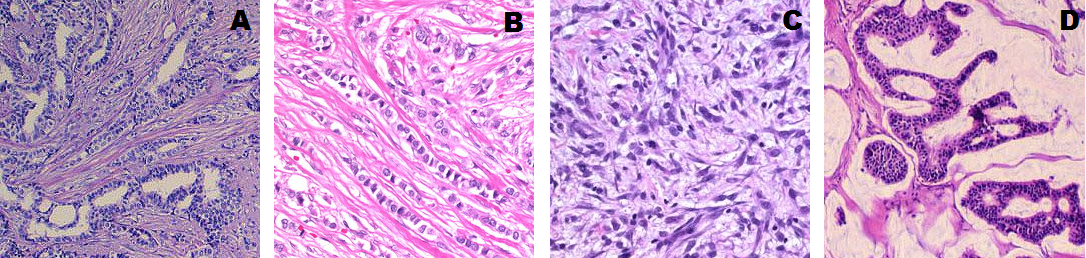
\includegraphics[scale=0.5]{morphology_labelled.png}
            \caption[Breast carcinoma invasive morphologies/histologies.]{Breast carcinoma invasive morphologies/histologies. (A) Ductal, (B) Lobular, (C) Metaplastic, (D) Mucinous. Images taken from \cite{Ramnani2016Webpathology.com:Images, Abdelmessieh2016BreastOverview}}
            \label{fig:histology}
            \end{figure} 
    
  IDC and ILC have distinct pathological features. Specifically, lobular carcinoma small cells are arranged individually, in single sheet pattern, and they have different molecular and genetic aberrations that distinguish them from ductal carcinomas \cite{weigelt2010molecular}. The lobular phenotype is determined by dyregulation of cell-cell adhesion, primarily driven by lack of \textit{E}-cadherin protein expression, which is often used as staining marker to tell it apart from the ductal morphology\cite{Ciriello2015ComprehensiveCancer, Abdelmessieh2016BreastOverview}. Ductal carcinoma has no specific histological characteristics other than invasion through the basement membrane of a breast duct \cite{Weigelt2008RefinementTypes}. 
   
    Metaplastic and mucinous carcinomas are very rare types of breast carcinomas that account for $>1\%$ and $2\%$ of all cases  \cite{Makki2015DiversityRelevance}. 
    Metaplastic breast cancer is a histologically distinct type due to its characteristic outlook of complex admixture of differentiated cells  \cite{Makki2015DiversityRelevance}. It is made up of abnormally looking ductal-origin cells which are thought to have undergone a change in form (\textit{metaplasia}) to become completely different cells that look like soft and connective tissue in the breast. Metaplastic breast cancers are also known to  behave more aggressively than other kinds of breast cancers \cite{schwartz2013metaplastic}. 
    It has been show that $>90\%$ of these cancers lack expression of ER/PR and HER2 (i.e. triple negative), and display a basal-like molecular profile \cite{Weigelt2010a} (more detail in the following sections).


    Mucinous carcinoma is less aggressive than more typical kinds of invasive cancer. The histological hallmark of this carcinoma is the excess of extracellular mucin, which surrounds the cancer cells and becomes part of the tumour \cite{dumitru2015mucinous}.  Mucinous tumours are usually ER/PR positive and HER2 negative, and consistently display a luminal phenotype \cite{Weigelt2010a}. 
    

   
    \subsubsection{Receptor Status}
    
    The identification of breast cancer receptor status is routinely used for prognostic and predictive  purposes \cite{Zaha2014}. A prognostic factor aims to give an indication of patient's overall clinical outcome (i.e. risk of recurrence and mortality), while a predictive factor is any measurement associated with response to a given therapy \cite{cianfrocca2004prognostic}. 
    
    The most common method of testing for receptor status is immunohistochemistry (IHC), which stains the cells based on the presence of estrogen receptors (ER), progesterone receptors (PR) and  human epidermal growth factor receptor 2 (HER2) \cite{Zaha2014}. Receptor status is a critical assessment for all breast cancers as it determines the suitability of using targeted adjuvant treatments such as tamoxifen and trastuzumab, which are now one of the most effective treatments of breast cancer \cite{stickeler2011prognostic}. 

    Approximately 70\% of invasive breast cancers are ER and/or PR positive. Estrogen and/or progesterone receptor positive cancer cells depend on estrogen or related hormones for their growth, therefore this kind of cancer can be treated with endocrine therapy drugs to reduce either the effect of estrogen (e.g. tamoxifen) or the actual levels of estrogen itself \cite{early2005effects}. In this way, hormone therapy blocks the tumour from using estrogen and/or progesterone thereby slowing or stopping its growth. 

    15-20\% of invasive breast cancers are characterised by overexpression of HER2  \cite{stickeler2011prognostic}, which is a good example of both a prognostic and predictive biomarker. HER2 expression is associated with a worse prognosis and higher risk of recurrence, however, HER2+ patients can immensely benefit from the highly effective therapeutic option such as the monoclonal antibody therapy (trastuzamab) \cite{iqbal2014human}. 

    Cancers that do not express any of the three receptors (ER, PR, HER2) are referred to as triple-negative breast cancers (TNBC) \cite{foulkes2010triple}. Triple-negative breast cancers comprise a very heterogeneous group of cancers, with a variety of prognoses, but often are associated with a more aggressive outlook. These cancers are the most challenging type, because they do not respond to endocrine therapy or other available targeted agents \cite{hudis2011triple}. 

    
    
    
    
    
    
    
            
 
            
    \subsubsection{PAM50 Molecular Profile}
    

With the wider adaptation of high-throughput gene expression profiling, it has been shown that tumour cell response to treatment is determined by ‘molecular profiles’ rather than physiological tumour characteristics and receptor status \cite{Weigelt2010}. 

The original studies by Sørlie \textit{et al.} \cite{Srlie2001GeneImplications} classified breast cancer tumours into five intrinsic subtypes with distinct clinical outcomes based on their ‘molecular portrait’: Luminal A, Luminal B, Basal-like, HER2-overexpressed, and Normal-like. The classification was guided by the differences underlying the gene expression patterns that reflect the fundamental differences of the tumours at the molecular level \cite{Srlie2003RepeatedSets}. The observed five subtypes map quite well to the previously defined IHC receptor subtypes (Table  \ref{table:pam50summary}), and have been repeated by several other studies with varying number of genes included in the subtypes’ signature \cite{Dai2015}. 

In 2009, Parker \textit{et al. }\cite{ParkerSupervisedSubtypes} reported a clinically applicable 50-gene classifier, PAM50, containing mostly hormone receptor and proliferation-related genes. By comparing global gene expression data from microarray and qRT-PCR, a minimized set of 50 genes was identified that could reliably classify each tumour into one of the intrinsic subtypes with 93\% accuracy. Over the past 7 years, the PAM50 intrinsic subtypes have shown to provide significant prognostic and predictive information beyond standard clinicopathological parameters \cite{Vidal2017} \cite{GnantPredictingAlone}. The PAM50 assay is now clinically implemented worldwide using the \textit{nCounter} platform \cite{Vidal2017}.

\begin{table}[!h]
\centering
\caption[Summary of the breast cancer molecular subtypes.]{Summary of the breast cancer molecular subtypes. PAM50 subtypes map to IHC status subtypes. Ki67 proliferative marker is used as a distinction between Luminal A and B. Luminal A and Normal-like share the IHC subtype. \textit{Table adapted from \cite{Dai2015}.}}
\label{table:pam50summary}
\begin{tabular}{l|c|l}
\multicolumn{1}{c|}{\textbf{PAM50  subtype}} & \textbf{IHC receptor status} & \multicolumn{1}{c}{\textbf{Prognosis}} \\ \hline
\multicolumn{1}{|l|}{Luminal A} & {[}ER+PR+{]} HER2- Ki67- & \multicolumn{1}{l|}{\textit{Good}} \\ \hline
\multicolumn{1}{|l|}{\multirow{2}{*}{Luminal B}} & {[}ER+PR+{]} HER2- Ki67+ & \multicolumn{1}{l|}{\textit{Intermediate}} \\ \cline{2-3} 
\multicolumn{1}{|l|}{} & {[}ER+PR+{]} HER2+ Ki67+ & \multicolumn{1}{l|}{\textit{Poor}} \\ \hline
\multicolumn{1}{|l|}{HER2-enriched} & {[}ER-PR-{]} HER2+ & \multicolumn{1}{l|}{\textit{Poor}} \\ \hline
\multicolumn{1}{|l|}{Basal-like} & {[}ER-PR-{]} HER2-, basal marker & \multicolumn{1}{l|}{\textit{Poor}} \\ \hline
\multicolumn{1}{|l|}{Normal-like} & {[}ER+PR+{]} HER2- Ki67- & \multicolumn{1}{l|}{\textit{Intermediate}} \\ \hline
\end{tabular}
\end{table}
    

\textbf{Luminal tumours}\\
Luminal A and B subtypes are distinguished by the expression of two main biological processes: proliferation/cell cycle-related pathways and luminal/hormone-regulated pathways \cite{Vidal2017}, and have expression patterns reminiscent of the luminal component of the breast \cite{perou2000molecular}. Luminal tumours are the most common subtypes among breast cancer (~60\%) with Luminal A being the majority \cite{Dai2015}.  Luminal A is characterised by expression of ER-related genes and low expression of proliferative genes, which is conversely high in Luminal B \cite{eroles2012molecular}. The IHC profile for Luminal A includes positive expression of ER, PR, cytokeratin CK8/18, and absence of HER2 expression and low Ki67 (proliferation marker) \cite{Vidal2017}. Luminal B tumours have higher expression of proliferation related genes, and lower expression of luminal-related genes or proteins such as PR and FOXA1, but not ER \cite{prat2012prognostic}, which is found similarly expressed between two luminal subtypes and can only help distinguish luminal from non-luminal disease \cite{Vidal2017}.

In general, the luminal subtypes carry a good prognosis, with Luminal B tumours having a significantly worse scenario than the Luminal A \cite{Srlie2003RepeatedSets}. Treatment response differs between the two, but generally they respond well to hormone therapy and poorly to conventional chemotherapy \cite{brenton2005molecular}. Luminal A tumours could be adequately treated with endocrine therapy, while luminal B tumors which are more proliferative may benefit more from the combined therapeutic strategy of chemotherapy and hormonal treatment \cite{paik2004multigene}.\\


\textbf{HER2-enriched tumours}\\
The identification of HER2-enriched subtype among the molecular profiles found in breast cancer was reassuring because it confirmed the clinical impression that the tumours with HER2 overexpression are systematically different from other breast cancers \cite{brenton2005molecular}. 
The HER2-enriched subtype is characterised by the high expression of HER2-related and proliferation-related genes, intermediate expression of luminal-related genes, and low expression of basal-related genes and proteins \cite{Vidal2017}. The best mapping IHC subtype to HER2-enriched tumours is HER2-overexpressed  (ER-/PR-/HER+), but it is not exclusive to them, i.e. it can be associated with other subtypes too \cite{Dai2015}. Additionally, although the majority (68\%) of HER2-enriched tumours have HER2 amplification, there are also cases of HER2-enriched subtype with HER2 negative receptor status \cite{Vidal2017}.

HER2-enriched tumours carry poor prognosis that is derived from a higher risk of early relapse \cite{carey2007triple}, but they can benefit greatly targeted therapeutic agents, such as anti-HER2 monoclonal antibody trastuzumab. \\


\textbf{Basal-like tumours}\\
The Basal-like subtype name comes from the observation that the expression pattern of this subtype resembled that of the basal epithelial cells of other parts of the body and normal breast myoepithelial cells \cite{perou2000molecular, brenton2005molecular}. The characteristics include lack of expression of ER-related (luminal) genes, low expression of HER2, and strong expression of basal markers (such as cytokeratins 5, 6, 17) \cite{sotiriou2003breast}. Some of the important hallmarks of basal phenotype is low expression of BRCA genes \cite{callagy2003molecular} and aggressive features such as TP53 mutations \cite{Srlie2001GeneImplications}. 

Among all the intrinsic subtypes, Basal-like is the most distinct \cite{TCGAComprehensiveTumors}. The unsupervised results in 2013 study by Prat \textit{et al.} \cite{prat2013genomic}  revealed that a subgroup of breast cancers, Basal-like by PAM50, should be considered a molecular entity by itself just like ovarian or colorectal cancer, and that $>70\%$ of basal-like breast cancers were more similar to squamous cell lung cancer than to Luminal A or B disease \cite{prat2013genomic}. 

Basal-like tumours account for 60-90\% of triple negative breast cancers \cite{fan2006concordance}, and in the past the terms TNBC and Basal-like were used interchangeably \cite{Vidal2017}. However, within TNBC, all intrinsic molecular subtypes can be identified. 
Triple negative Basal-like tumours are of particular interest because of their aggressive clinical course and currently lack any form of standard targeted systemic therapy. These tumors are associated with a lower disease-specific survival and a higher risk of local and regional relapse \cite{hudis2011triple}. 
The size of basal tumors is, in general, larger than the other subtypes\cite{rakha2006morphological}, and they also tend to show rapid growth \cite{ho2012characterization}. The metastasis pattern also separates basal tumors from the other breast cancers, with a tendency towards internal organs (excluding bone) and less likely to involve lymph nodes \cite{ho2012characterization}. 
.
The poor prognosis of basal-like subtype  has been confirmed by multiple independent data \cite{brenton2005molecular}. However, it is not clear if this prognosis is due to poor therapy options or inherent aggressiveness. Given the triple negative receptor status,  basal tumors are not amenable to conventional targeted breast cancer therapies such as endocrine therapy or trastuzumab, leaving chemotherapy the only option \cite{brenton2005molecular, Dai2015}. \\


\textbf{Normal-like tumours }\\
Normal-like intrinsic subtype is the smallest breast cancer group that accounts for less than 10\% of the cases \cite{Dai2015}. Normal-like subtype shares its IHC receptor status with Luminal A ([ER+ PR+] HER2- Ki67-), but differs on expression pattern. Also, as suggested by the name, Normal-like cancers are characterised by a normal breast tissue profiling \cite{perou2000molecular}. Still, while normal-like breast cancer has a good prognosis, its prognosis is slightly worse than Luminal A cancer’s prognosis.\\





\textbf{final words}

























    \newpage    
    \subsection{The Cancer Genome Atlas}
    
    
    
    \subsubsection{Purpose and Organisation}

    The Cancer Genome Atlas (TCGA) network \cite{TheTCGA}, a collaboration between the National Cancer Institute (NCI) and National Human Genome Research Institute (NHGRI), and a part of NCI Genomic Data Commons (GDC) portal from 2016 \cite{NCICommons}, maintains a public database of clinical and molecular data over 33 different tumour types with hundreds of cases per type, making it the most comprehensive repository of human cancer data \cite{OverviewTCGA}. Over the past decade TCGA research network has generated and maintained 2.5 petabytes of data describing tumour and matched normal tissues from more than 11,000 patients that is publicly available and has been used widely by the research community \cite{OverviewTCGA}. The data have contributed to more than a thousand studies of cancer by independent researchers and to the TCGA research network publications \cite{Editorial.2015TheGenomics}.

    The structure of TCGA is well organised and involves several cooperating centres responsible for collection and sample processing, followed by high-throughput sequencing and bioinformatics data analyses \cite{Tomczak2015TheKnowledge, OverviewTCGA}. The generated data is made available to the research community through public free-access databases such as NCI GDC data portal, GDC Legacy Archive and the Broad Institute’s Firehose \cite{PapaleoTCGAPackages}. \\To provide comprehensive analysis of cancer genome profiles, the TCGA research network works with many centres utilising different platforms to provide global information of cancer genomics, including high-throughput technologies based on microarrays and next-generation sequencing methods. Some of the applied methods include: RNA-sequencing, miRNA-sequencing, exon sequencing, SNP genotyping, DNA methylation profiling, Reverse-phase protein array (RPPA) \cite{OverviewTCGA}. The multidimensional analyses performed on distinct platforms provide scientists with better understanding of cancer biology, leading to improved cancer classification, development of new diagnostic methods and therapeutic approaches.\\



    \subsubsection{Data Access}

    Two versions of TCGA data are available: harmonised and legacy. The harmonised data is accessible via the NCI GDC data portal \cite{NCICommons}, and it represents a subset of the full TGCA data that has been harmonised against GRCh38 (hg38) using GDC Bioinformatics Pipelines. The GDC Legacy Archive provides access to an unmodified copy of data that was previously stored in the TCGA Data Portal hosted by the TCGA Data Coordinating Center (DCC), and  which uses as references GRCh37 (hg19) and GRCh36 (hg18) \cite{PapaleoTCGAPackages}.

    The legacy data is provided as different levels that are defined in terms of a specific combination of both processing level (raw, normalised, integrated) and access level (controlled or open access), while the GDC open access data does not require authorisation to access the high level genomic data that is not individually identifiable \cite{NCICommons, PapaleoTCGAPackages}.
    
    Finally, the data provided by GDC data portal and GDC Legacy Archive can be accessed using R/Bioconductor package TCGAbiolinks \cite{Colaprico2016}. The Bioconductor project ensures high-quality, well-documented and interoperable software and the possibility of integration with hundreds of available packages within R, and is a highly valuable bioinformatics resource \cite{gentleman2004bioconductor}. \\TCGAbiolinks aids in querying, downloading, pre-processing, and analysing TCGA within a single package, allowing user to have a better control over the data and making the results to be easily reproducible \cite{Colaprico2016}. The full clinical report and molecular data (quantified by a variety of methods mentioned above) are prepared to download into a ‘SummarizedExperiment’ object \cite{Huber2015OrchestratingBioconductor}, which allows easy integration with other data types and statistical methods that are common in the Bioconductor repository.  In line with that, the TCGAbiolinks package has a variety of incorporated methodologies for processing and filtering the data.  
    
    \newpage
    \subsubsection{Breast Cancer Dataset}
    
    TGCA breast cancer dataset (TCGA-BRCA) is the largest by number of patients cancer type dataset available in TCGA. One of the most complete breast cancer characterisation studies that has ever been performed is the 2012 TCGA research network study \cite{TCGAComprehensiveTumors} that succeeded to identify comprehensive molecular portraits of human breast tumours. 
    
    In this study, around 500 primary breast cancers were extensively profiled at the DNA (i.e., methylation, chromosomal copy number changes, and somatic and germ line mutations), RNA (i.e., miRNA and mRNA expressions), and protein (i.e., protein and phosphorprotein expression) levels using the most recent technologies \cite{TCGAComprehensiveTumors, Vidal2017}.
    
    By classifying tumours using each individual platform and comparing results at different levels through combining the data together in a cluster of clusters, they concluded that diverse genetic and epigenetic alterations converge phenotypically into four major breast tumour subgroups \cite{TCGAComprehensiveTumors}. But also importantly, these four entities were found to be recapitulated very well by the four main intrinsic subtypes (Luminal A, Luminal B, HER2-enriched, and Basal-like) as previously defined by mRNA expression only in the Parker’s study \cite{ParkerSupervisedSubtypes}. The Normal-like subtype had limited amount of samples, and therefore was not rigorously explored. Overall, these results suggested that intrinsic subtyping captures a great amount of biological diversity that occurs in breast cancer. 
    
    Another large-scale TCGA-BRCA study was conducted by Ciriello \textit{et al.} in 2015 \cite{Ciriello2015ComprehensiveCancer} on profiling 817 breast cancer samples. The study had a much larger proportion of lobular carcinoma tumours than the original TCGA work, where those were underrepresented. The study shed new light on the genetic bases of lobular morphology and provided more insights into the intrinsic subtypes and their distribution across different morphologies. 
    
    
    
   
    
    
    
    




    
    
    
    
    
    
    
    
    
        
        
        
     \newpage   
    \subsection{Autophagy}
    % In 2016, a Nobel Prize in Physiology or Medicine was given to Prof Yoshinori Ohsumi (Anon n.d.), a renowned scientist in the autophagy research field, for his success in elucidating the sophisticated machinery of the autophagy pathway. Because of his pioneering work, autophagy is recognized as a fundamental process in cell physiology with major implications for human health and disease. 
    % Autophagy is an evolutionarily conserved lysosomal degradation process that is crucial for adaptation to stress and maintaining cellular homeostasis (Feng et al. 2015). Recent studies have demonstrated association between autophagy and cancer, which implies that autophagy plays an important role in the development, progression, and response of breast cancer cells to chemotherapy and other therapies (Debnath n.d.). 
    
    % Upon starvation or stress conditions, autophagy is induced. Damaged organelles and cytoplasm are sequestered by an expanding phagophore, leading to the formation of double-membrane autophagosome (Feng et al. 2015), as shown in Figure 2. The autophagosome subsequently fuses with the lysosome, followed by the degradation of the sequestered cargo (Yorimitsu and Klionsky 2005). Then, the breakdown products are released back in cytosol through permeases. This allows recycling of the macromolecular constituents as building blocks, to generate energy to maintain cell viability under unfavourable conditions (Feng et al. 2013). 
    % Autophagy is involved in normal aspects of cell development and physiology, and defects in this process are associated with a range of diseases, including cancer. The work of Ohsumi and the colleagues has led to identification several dozens of autophagy-related genes, allowing for targeted research aimed at  understanding of the autophagy mechanisms, with the ultimate goal to manipulate or target them for therapeutic purposes (Feng et al. 2015). 


        \subsubsection{a}
        \subsubsection{b}


        
        
        
        
        
    \subsection{Autophagy in Cancer}
    % The role of autophagy in tumorigenesis and treatment response is complicated and context-dependent, and presumed to differ between stages of cancer progression (Zarzynska and Magdalena 2014). Autophagy’s role in maintaining organelle and protein turnover allows cells to restrain damage, including genome instability and inflammation, thereby limiting initiation and progression of cancer at early stages. However, once tumour develops, the cancer cells are able to utilize autophagy for their own cytoprotection (Zarzynska and Magdalena 2014). Autophagy is believed to promote cancer by allowing cells to survive under conditions of metabolic and genotoxic stress (Mathew and White n.d.). Unfavourable conditions such as hypoxia and acidity in tumour environment as well as the effects of chemo- and radiotherapy cause cells to experience stress and nutrient deprivation (Bailey et al. n.d.). Induction of autophagy within these cells allows them to survive the drastic conditions. This kind of mechanism had been referred to as “what doesn’t kill you, makes you stronger” by researchers in the field (Mathew and White n.d.).
        \subsubsection{a}
        \subsubsection{b}
        
        
        


\section{Thesis objectives}
% The role of autophagy in tumorigenesis and treatment response is complicated and context-dependent, and presumed to differ between stages of cancer progression (Zarzynska and Magdalena 2014). Autophagy’s role in maintaining organelle and protein turnover allows cells to restrain damage, including genome instability and inflammation, thereby limiting initiation and progression of cancer at early stages. However, once tumour develops, the cancer cells are able to utilize autophagy for their own cytoprotection (Zarzynska and Magdalena 2014). Autophagy is believed to promote cancer by allowing cells to survive under conditions of metabolic and genotoxic stress (Mathew and White n.d.). Unfavourable conditions such as hypoxia and acidity in tumour environment as well as the effects of chemo- and radiotherapy cause cells to experience stress and nutrient deprivation (Bailey et al. n.d.). Induction of autophagy within these cells allows them to survive the drastic conditions. This kind of mechanism had been referred to as “what doesn’t kill you, makes you stronger” by researchers in the field (Mathew and White n.d.).



\chapter{Methods}
%\section{Data}
    \subsection{Data sources}
    
    The full TCGA-BRCA RNA-sequencing dataset was downloaded from the GDC data portal using R/Bioincuctor package TCGAbiolinks v2.8.13
\cite{Colaprico2016}. Table \ref{table:full} shows the overview of samples collected by the TCGA research network. 

     %   TABLE 2.1
            \begin{table}[!htbp]
                \centering
                \caption{TCGA-BRCA full dataset sample number overview}
                \label{table:full}
                    \begin{tabular}{c|c|c|c}
                    \textbf{Samples} & \textbf{Tumour} & \textbf{Normal} & \textbf{Metastasis} \\ \hline
                    \multicolumn{1}{|c|}{\begin{tabular}[c]{@{}c@{}}1212 \\ (F:1199, M:13)\end{tabular}} & \begin{tabular}[c]{@{}c@{}}1093\\ (F:1082, M;12)\end{tabular} & \begin{tabular}[c]{@{}c@{}}112\\ (F: 111, M:1)\end{tabular} & \multicolumn{1}{c|}{\begin{tabular}[c]{@{}c@{}}7\\ (F:7, M:0)\end{tabular}} \\ \hline
                    \end{tabular}
            \end{table}

    The original dataset has been subset to a more manageable collection of samples based of three main factors, which entailed including samples that \textbf{ i)} are female only (to reduce biological variation coming from gender) \textbf{ii)} are present in the list of manually curated samples and their classifications \textbf{iii)} are provided with enough metadata to benefit exploratory analysis. Only primary tumour and normal samples were included in the analysis.
    
    The curated lists of samples specifying stage and morphological type of samples were provided by the collaborators from other groups at DCRC.Table \ref{table:morphstage} shows the number of samples that were represented in the morphological groups and stages in the final dataset. 
    
    
     %   TABLE 2.2
            \begin{table}[!htbp]
            \centering
            \caption{The number of samples in each morphology type and stage in the final datset}
            \label{table:morphstage}
            \begin{tabular}{lccllclc}
            \multicolumn{1}{c}{\textbf{Morphology}} & \textit{\begin{tabular}[c]{@{}c@{}}ICD-O-3 \\ code\end{tabular}} & \textbf{} &  &  & \textbf{} & \multicolumn{1}{c}{\textbf{Stage}} & \textbf{} \\ \cline{1-3} \cline{7-8} 
            \multicolumn{1}{|l|}{Lobular Carcinoma} & \multicolumn{1}{c|}{8520/3} & \multicolumn{1}{c|}{100} &  &  & \multicolumn{1}{c|}{} & \multicolumn{1}{l|}{stage 1} & \multicolumn{1}{c|}{100} \\ \cline{1-3} \cline{7-8} 
            \multicolumn{1}{|l|}{Infiltrating Duct Carcinoma} & \multicolumn{1}{c|}{8500/3} & \multicolumn{1}{c|}{100} &  &  & \multicolumn{1}{c|}{} & \multicolumn{1}{l|}{stage 2} & \multicolumn{1}{c|}{100} \\ \cline{1-3} \cline{7-8} 
            \multicolumn{1}{|l|}{Infiltrating Duct and Lobular Carcinoma} & \multicolumn{1}{c|}{8522/3} & \multicolumn{1}{c|}{100} &  &  & \multicolumn{1}{c|}{} & \multicolumn{1}{l|}{stage 3} & \multicolumn{1}{c|}{100} \\ \cline{1-3} \cline{7-8} 
            \multicolumn{1}{|l|}{Metaplastic carcinoma} & \multicolumn{1}{c|}{8575/3} & \multicolumn{1}{c|}{100} &  &  & \multicolumn{1}{c|}{} & \multicolumn{1}{l|}{stage 4} & \multicolumn{1}{c|}{100} \\ \cline{1-3} \cline{7-8} 
            \multicolumn{1}{|l|}{Mucinous adenocarcinoma} & \multicolumn{1}{c|}{8480/3} & \multicolumn{1}{c|}{100} &  &  & \multicolumn{1}{c|}{} & \multicolumn{1}{l|}{stage X} & \multicolumn{1}{c|}{100} \\ \cline{1-3} \cline{7-8} 
            \multicolumn{1}{|l|}{Other morphologies} & \multicolumn{1}{l|}{} & \multicolumn{1}{c|}{100} &  &  &  & \multicolumn{1}{c}{} &  \\ \cline{1-3}
            \end{tabular}
            \end{table}
    
    
    Each sample in the final dataset was annotated with clinical metadata, which included PAM50 molecular subtype, patient age subgroup, race/ethnicity, menopause status, tumour grade, nodal involvement, metastasis status, year sample was taken, tissue source site. 
    The metadata for each sample was collected and integrated from three sources. The sample annotations extracted with TCGAbiolinks was complimented with the additional subtype classifications for the previously unclassified samples from a recent TCGA-BRCA study by Ciriello \textit{et al.} \cite{Ciriello2015ComprehensiveCancer}. Further metadata was added from the work by Rahman \textit{et al. }\cite{RahmanAlternativeResults} on reprocessing TCGA data. \\   
    
        
    A curated collection of autophagy-related gene lists was provided by experts in the field at DCRC (in the Cell Death and Metabolism and Cell Stress and Survival Units). Table \ref{table:autophagy} shows the functional groups that autophagy-related genes are managed by. The autophagy core genes and as well as transcription factors are of the most interest. 
    
     %   TABLE 2.3
    
            \begin{table}[!htbp]
            \centering
            \caption{Autophagy-related genes functional groups. The numbers are reported for the dataset after pre-processing.}
            \label{table:autophagy}
            \begin{tabular}{l|c}
            \textbf{Functional Group} & \multicolumn{1}{l}{\textbf{Number of genes}} \\ \hline
            Autophagy core & 156 \\ \hline
            Transcription factors & 101 \\ \hline
            Lipid & 33 \\ \hline
            Phosphatidyl & 40 \\ \hline
            Endo and exosomes & 132 \\ \hline
            Transport & 216 \\ \hline
            RABs and effectors & 131 \\ \hline
            Docking and fusion & 14 \\ \hline
            Mitophagy & 65 \\ \hline
            Receptors and ligands & 66 \\ \hline
            mTOR induction & 138 \\ \hline
            Lysosome & 218 \\ \hline
            \multicolumn{1}{c|}{\textit{Total}} & \textit{1112}
            \end{tabular}
            \end{table}
            
            
    \subsection{Data quantification, extraction, and preprocessing}
    The original RNA-seq data was quantified by University of North Carolina (UNC) Center for Bioinformatics for the TCGA project \cite{UniversityofNorthCarolinaUNCCenterforBioinfromatics2013TCGAData}. The quantification pipeline included  using Mapsplice v12.07 \cite{wang2010mapsplice} for mapping the data to reference genome (GRCh37/hg19), RSEM v1.1.13 \cite{li2011rsem} for transcript quantification \cite{UniversityofNorthCarolinaUNCCenterforBioinfromatics2013TCGAData}. 

    The TCGA portal datasets for different cancer types are accessible at three levels: 1) raw and uncontrolled, 2) normalised and controlled, and 3) integrated and interpreted. In this project, level 2 Legacy Breast Cancer dataset was downloaded and prepared using the TCGAbiolinks preprocessing pipeline. The pipeline contains integrated functions from the EDASeq package \cite{risso2011gc} for within-lane normalisation procedures to adjust for GC-content and gene length effects on read counts, as well as between-lane normalisation method to adjust for distributional differences between lanes (e.g. sequencing depth), such as quantile normalisation (cut-off 0.10)\cite{Colaprico2016, PapaleoTCGAPackages}.  The pipeline transforms the data into a '\textit{SummarizedExperiment}' \cite{Huber2015OrchestratingBioconductor} object (counts table), with genes and samples as rows and columns, respectively. 
    
    
    \subsection{Final dataset}
    
    After data pre-processing and filtering for samples with sufficient clinical information, the final dataset included 969 tumour and 112 normal samples, and  the gene expression matrix was reduced to 17372 genes. 
    All samples were annotated with PAM50 molecular classification. Table \ref{pam50counts} shows the sample counts for each PAM50 subtype. 
    
    
     %   TABLE 2.4    
                \begin{table}[!htbp]
                \centering
                \caption{The number of samples in each PAM50 subtype in the final dataset}
                \label{pam50counts}
                \begin{tabular}{ll}
                \multicolumn{1}{c}{\textbf{PAM50}} &  \\ \hline
                \multicolumn{1}{|l|}{Luminal A} & \multicolumn{1}{l|}{100} \\ \hline
                \multicolumn{1}{|l|}{Luminal B} & \multicolumn{1}{l|}{100} \\ \hline
                \multicolumn{1}{|l|}{Basal-like} & \multicolumn{1}{l|}{100} \\ \hline
                \multicolumn{1}{|l|}{HER2-enriched} & \multicolumn{1}{l|}{100} \\ \hline
                \multicolumn{1}{|l|}{Normal-like} & \multicolumn{1}{l|}{100} \\ \hline
                \end{tabular}
                \end{table}
                
    
    %table with all classifications, descripron of SE and sample matrix; other metadata available for majority od samples 
    
    
\section{Exploratory analysis methods}
    % paragraph avout EDA and how it is need before hypothesis-driven analysis
    
    Exploratory data analysis (EDA) is an essential step in working with a large dataset of publicly available data, such as the TCGA-BRCA dataset. Exploratory analysis can be applied to raw and normalised transcriptomics data as a means to visualise the global structure of the data. Metadata available for all samples was rigorously explored to maximise the insight into the dataset, extract important features, and to highlight outliers and potential confounders.
    
    Principal component analysis (PCA) and clustering (as part of a heatmap and not) are the most commonly used exploratory tools. The underlying statistics and algorithms available for the calculations involved in PCA and clustering dendogram generation are fundamentally the same for the available packages in R/Bioconductor. This section will present a general introduction to PCA and clustering, and provide simple examples of use.

    \subsection{Principal Component Analysis}
    
    PCA is a method that linearly transforms a multivariate dataset into a set of uncorrelated variables ordered in descending manner by the variance explained \cite{jolliffe2002principal}. In this way, the first few principal components (PCs) often explain the largest amount of the variation in the data. PCA results can be visualised in a 2D scatter plot, where $x$ and $y$ axes are the selected principal components. The samples are projected onto the 2D plane such that they spread out in the two directions that capture the most of the variance across samples \cite{Love2016RNA-SeqApproved}. 
    In a PCA 2D scatter plot, each data point represents a sample, which allows visualisation of sample clustering and dataset structure.  The relationship between two samples is reflected by the distance between corresponding dots in the plot. Therefore, the more similar gene expression profiles are, the closer the data points are.    
   
    Figure \ref{fig:pcamethod} shows an example of separation of transcriptional profiles of cancer (pink) and normal (blue) samples. The primary source of variation (PC1) accounts for 11\% of the total variation in the data. The second principal component (PC2) accounts for 8.6\% of the total variation in the data. PCA was performed using the R function \texttt{prcomp()}.
    
        % PCA plot 
            \begin{figure}[h]
            \centering
            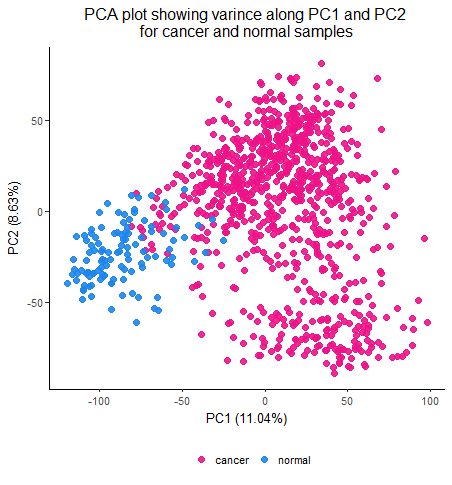
\includegraphics[scale=0.7]{pca_method.png}
            \caption{An example of PCA 2D scatter plot, showing the variance along PC1 and PC2 for cancer and normal samples}
            \label{fig:pcamethod}
            \end{figure}
        
    \newpage
    Another way of exploring variation characterised by PCA is to visualise variation of each principal component in a series of one-dimensional box plots. Figure \ref{fig:1dpcamethod} shows the variation seen in each PC (1-9) for the cancer/normal dataset shown as a scatter plot of first two PCs in Figure \ref{fig:pcamethod}. 
    In contrast, one-dimensional PCA plots are able to show variation along more than two PCs at a time. This method is useful for checking if any of the other PCs contain variation worth exploring. This is useful for checking for potential presence of batch effects or signatures left by other cofactors. 
    For each PC, the variation of each condition group, here - cancer and normal, is represented by a box plot. The PCs where condition boxes have the smallest overlap (e.g. PC1) will shows the clearest separation when plotted in 2D. 
       
    
        % PCA 1d
            \begin{figure}[h]
            \centering
            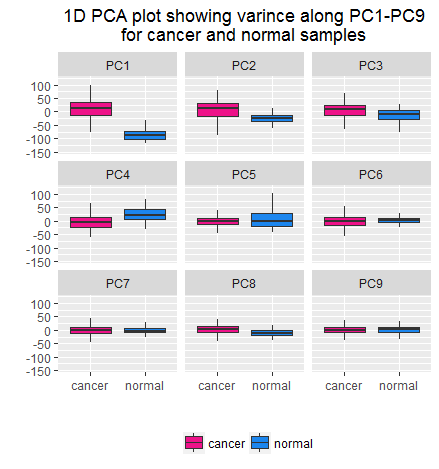
\includegraphics[scale=0.7]{1dpcamethod.png}
            \caption{An example of one-dimensional PCA plots for the cancer/normal dataset. }
            \label{fig:1dpcamethod}
            \end{figure}
   
  
    \subsection{Clustering and Heatmap representation}
    
    
    In clustering, or unsupervised classification, the aim is to identify subsets (clusters) in the data based on the similarity between single objects. Similar objects should be assigned to the same cluster, while objects which are not similar to each other, should be assigned to different clusters.
    Cluster analysis is applied to transcriptomics data to search for similar gene expression patterns between individual samples. This can help to reveal the data structure and give first insights into the data, which is especially useful if prior knowledge is little or non-existent. Clustering can, therefore, be seen as exploratory data analysis. 
        
    The purpose of clustering transcriptomics data is to statistically group samples according to their gene expression, in order to reduce complexity and dimensionality of the data, predict function or identify shared regulatory mechanisms \cite{Metsalu2015ClustVis:Heatmap}. Clustering can be performed as a part of heatmap. Heatmap is a datamatrix visualising values in the cells by the use of a color gradient. This gives a good overview of the largest and smallest values in the matrix. Rows (genes) and/or columns (samples) of the matrix are clustered to facilitate interpretation of sets of rows or columns rather than individual ones \cite{Metsalu2015ClustVis:Heatmap}.\\

    One of the popular methods is hierarchical clustering, which involves re-ordering of samples based on their distance in high dimensional space. The cluster is constructed based on the determination of two parameters — the distance metric and the linkage criterion.
    The two most common distance measures used for clustering are Euclidean and Manhattan distances. Typically the results of the two are quite similar, but most studies default to using the Euclidean measure. 
    The Euclidean distance involves computing the square root of square differences between two coordinates. In this way, the shortest path diagonally is calculated: $ \sqrt{(x_{1}-x_{2})^{2}+(y_{1}-y_{2})^{2}}$, where the first point is $(x1, y1)$ and the second point is $(x2, y2).$
    The Manhattan distance between two points is calculated by taking the sum of the lengths of the differences between the coordinates. Therefore, the distance is measure not in a straight line, but on horizontal (x) and vertical (y) axes — $ (x_{1}-x_{2})+(y_{1}-y_{2}).$
    
    Clustering works well when the data to be clustered is processed correctly. The low expressed genes have to be filtered out to remove non-informative noise after the counts data has been normalised and log2-transformed as will be discussed in section \ref{}, prior to clustering with the R function \texttt{hclust()} with default parameters. Hierarchical clustering on all genes was performed on all genes on data subgroup averages (Results section \ref{}).
    
    Heatmap clustering was performed on gene subsets, such as autophagy groups or $n$ genes with the highest variance (Results section \ref{}). The heatmaps were generated using Manhattan distance with avegare linkage (default) using the R package  \texttt{pheatmap} \cite{kolde2012pheatmap}.\\
    
    The results obtained for summarising the structure of transcriptomics data between PCA and clustering often show similar findings. For instance, if PCA shows a clear segregation of the data, clustering normally will support this.
    
    
    
%     HCL implementing the Euclidean distance metric and the average linkage
% distance method to analyse the same data used to generate the PCA in figure 6
% determines that the data clusters into two predominant groups — one comprising
% all cancer samples and the other consisting of all control (healthy) samples. This
% indicates that the cancer transcriptomic profiles are more similar to each other
% than any of the control samples. These findings are reflected by those obtained
% from the PCA.
    
\newpage



\section{Hypothesis-driven analysis methods}    

    %why

    \subsection{Differential Expression Testing}
    
    %why
        \subsubsection{data preprocessing}
        \subsubsection{DE background}
        \subsubsection{limma}
        \subsubsection{multiple tesing correction}

    \subsection{Soft clustering}
        \subsubsection{prepossessing}
    
    \subsection{Enrichment Analysis}
    
    \subsection{PPi, TF, miRNA networks}

\chapter{Results}
%    
\section{Exploratory Analysis}

    %data was preprocessed as described in methods
    
    
    % The outcome of the EDA will have a major impact on how you analyze the data:
    %  – Sample outliers and noise: Should some samples be discarded?
    % Can I perform a meaningful test for different expression between different groups?
    % What factors (wanted/unwanted, observed/unobserved) should be included in the model?
    
    % • EDA is the first part of the analysis where you start drawing biological conclusions specific to a
    % given experiment.
    % – Does the data look like I expected/designed?
    % – Do I have batch effects?
    % – Subgroups?
    % • In DE you formalize your observations in the EDA to extract statistically valid results.
    % • The resulting DE analysis will serve as the foundation of biological interpretation of the data.

    
    

    \subsection{Main effect subgroups}

    There are three main effects by which breast cancer samples can be stratified into groups: morphology, stage and PAM50 molecular profile. PCA is able separate samples into tumour/normal sample clusters fairly well (shown as an example in Methods, Figure \ref{fig:pcamethod}. However, it is more interesting to apply PCA to explore variation coming from separating samples in different cancer classification groups.  
    
    PCA was applied to 969 samples (857T, 112N), which were divided into subgroups by three systematic effect groups (i.e. PAM50, tumour morphology, cancer stage), which subgroup sizes shown in Tables \ref{table:morphstage} and \ref{table:pam50counts}. \\
    Figure \ref{fig:pcapam50} shows the PCA plot of first two principal components, coloured by PAM50 molecular subtype groups. PC1 accounts for 11\% of the total variation in the data, and is driven by the differences between normal and cancer samples. PC2 accounts for 8.6\% of the variation, and characterises the variation among breast cancer subtypes. Firstly, Basal-like samples form a separate cluster (orange), which emphasises its complete dissimilarity at molecular level. Luminal A and Luminal B form a partially overlapping cluster (yellow and red), which is expected from the known similarities of these subtypes. HER2-enriched cluster (blue) is understandably located between Luminal B and Basal-like as it is known to share expression profiles with these two. And lastly, seeing Normal-like subtype (pink) overlapping with normal samples (green) as well as with Luminal A cancer subtype fits nicely with the fact that Normal-like subtype shares morphology with the former and IHC and molecular profile with the latter.    
    
    % PAM50 PCA plot 
            \begin{figure}[!h]
            \centering
            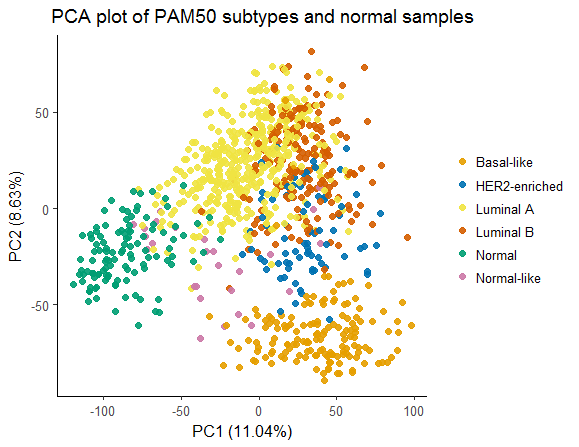
\includegraphics[scale=0.37]{pcapam502.png} 
            \caption{PCA plot showing the variance along PC1 and PC2 for PAM50 molecular subtypes of breast cancer and normal samples}
            \label{fig:pcapam50}
            \end{figure}
            
    \newpage
    Figure \ref{fig:1dpcapam50} shows the results of PCA for the first nine PCs, as described in the Methods section. Looking at the results in this way highlights again that PC1 is driven by tumour/normal variation. Together with PC2 they also capture the differences among PAM50 subtypes. As the PCs numbers increase, variation captured by them decreases. 
    
    % PAM50 1d PCA plot 
            \begin{figure}[!h]
            \centering
            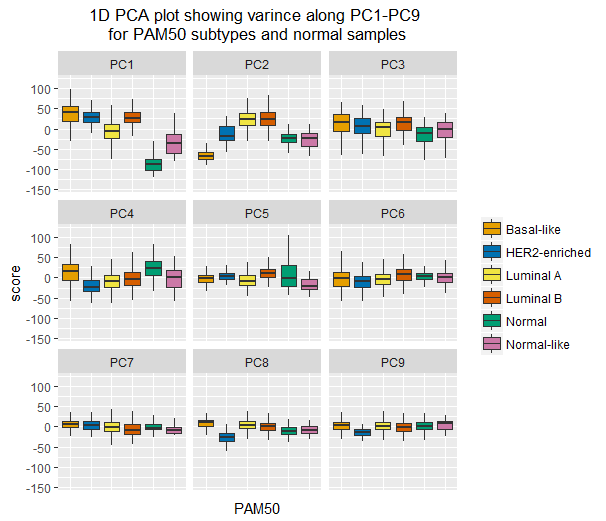
\includegraphics[scale=0.5]{1dpcapam50.png}
            \caption{One-dimensional PCA plots showing variance along PC1-PC9 for PAM50 molecular subtypes of breast cancer and normal samples. }
            \label{fig:1dpcapam50}
            \end{figure}
    
    
    The PCA results for morphology and stages classifications are shown in Figure \ref{fig:1dpcamorphstage} as one-dimensional variation plots. It can be observed that PCA was not able to capture as much variation between morphology groups and stages as among PAM50 subtypes. From one-dimensional plots it is evident that PC1 captures cancer/normal differences in both classification types. However, the rest of PCs do not capture enough variation to be evident on 2D PCA plots, therefore here only 1D plots are presented. Appendix \ref{} show 2D plots for results completion.    
    
    % 1D PCA for stages and morphology
            
            \begin{figure}[!h]
            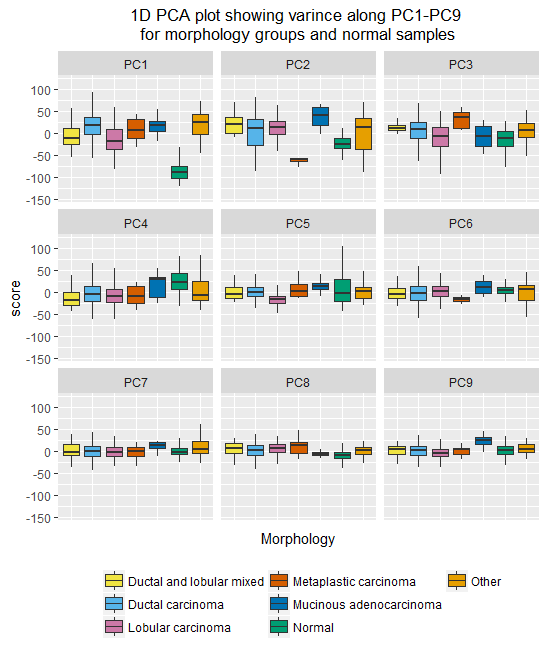
\includegraphics[width=0.4\linewidth]{1dpcamorph2.png}\hfill
            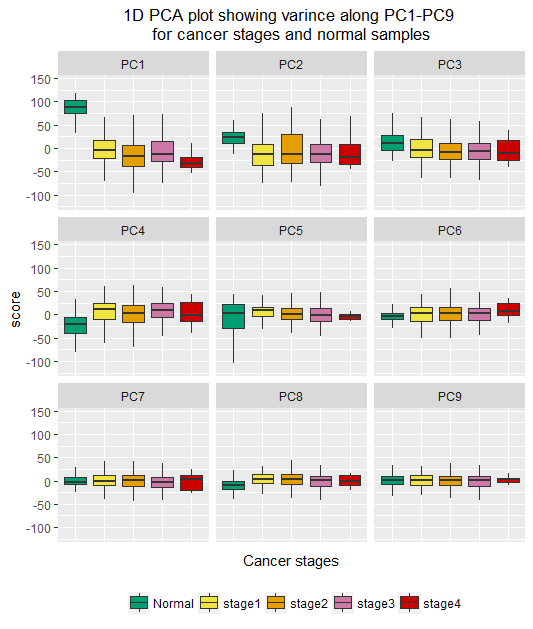
\includegraphics[width=0.4\linewidth]{1dpcastages2.png}
            \caption{One-dimensional PCA plots showing variance along PC1-PC9 for morphology groups and stages, with normal samples.}
            \label{fig:1dpcamorphstage}
            \end{figure}
            
    
    \newpage
    Interestingly, PCA was not able to capture any significant differences between stages (e.g. stage 1 and stage 4), where the differences in expression should be evident and therefore reflected in PCA results. The same is the case for two main distinct mythologies - Lobular and Ductal carcinomas, which overlap greatly. A possible explanation for these results is the unbalanced sizes of subgroups in these two classification methods, as well as their composition in terms of PAM50 subtypes, which is evidently the main driving force in sample classifications. 
    
    To explore this idea, the sample count data was visualised as stacked barplots presented in Figure \ref{fig:barms}. Each bar shows the total count of samples of a chosen morphology (left plot) or stage (right plot). The differing group sizes are evident.         
    
    % barsplots for stages and morphology 
       
        \begin{figure}[!h]
        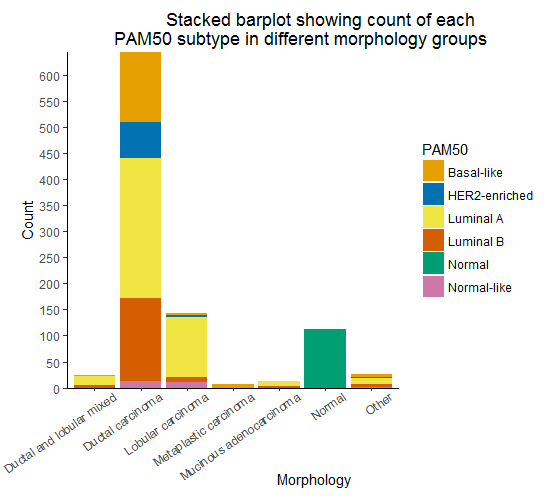
\includegraphics[width=0.53\linewidth]{bar_morph.png}\hfill
        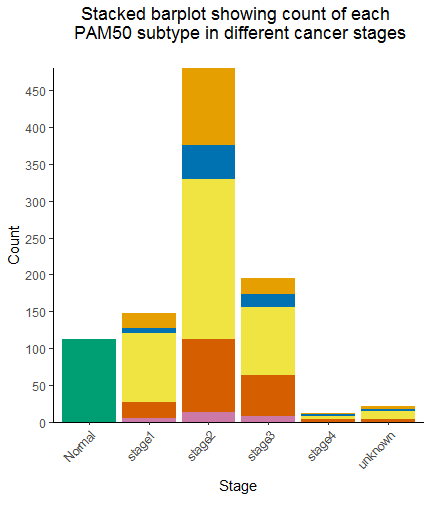
\includegraphics[width=0.4\linewidth]{bar_stages2.png}
        \caption{Stacked barplots of sample number counts per subgroups in morphology groups and stages classification groups. The coloured proportions represent PAM50 subtypes samples within each subgroup.}
        \label{fig:barms}
        \end{figure}
        
    Ductal carcinoma morphology samples make up over 70\% of all samples (x/857), but are well-proportionate in terms of PAM50 composition (i.e. similar proportions as the full dataset, with Luminal A dominating). Other subgroups, however, in addition to being smaller, are restricted to only a few PAM50 subtypes. For instance, Metaplastic carcinoma is made up completely of Basal-like samples, while Mucinous morphology is represented by only Luminal subtypes (the counts are shown in Table \ref{table:counts}). This observation explains why these two mophologies are separated in 1D PCA plot in PC2 (Figure \ref{fig:1dpcamorphstage}) - the difference between Luminal and Basal tissues is driving this variation. However, it is important to note, that there is a chance that these two morphologies, Metaplastic and Mucinous, actually only exists as Basal and Luminal subtype, respectively, but it is not possible to claim for or against this based on the current dataset.    
    
    The sample count difference between stages are also noticeable, which stage 2 accounting for roughly 50\% of the samples. The proportions of PAM50 subtypes within stages 1-3 appear to be well-balanced. Stage 4 is, however, of major concern. It has an alarmingly low sample count and is not represented in Normal-like subtype. The counts are shown in Table \ref{table:counts}.
        
        
    %TABLE x3 counts   
                \begin{table}[!h]
                \centering
                \caption{Samples number counts in pairwise comparisons of three main breast cancer samples classifications. Top table: PAM50 and stages, Middle table: PAM50 and morphology, Bottom table: stages and morphology. Each table shows row and column sums for each subgroup. The total count of samples in the project is in the lower right corner: 857.}
                \label{table:counts}      
                \resizebox{\textwidth}{!}{%
                \begin{tabular}{ccccccc}
                \multicolumn{1}{l|}{} & \multicolumn{1}{c|}{\textbf{Luminal A}} & \multicolumn{1}{c|}{\textbf{Luminal B}} & \multicolumn{1}{c|}{\textbf{Basal-like}} & \multicolumn{1}{c|}{\textbf{HER2-enriched}} & \multicolumn{1}{c|}{\textbf{Normal-like}} & {\color[HTML]{9B9B9B} \textit{rowsums}} \\ \hline
                \multicolumn{1}{c|}{\textbf{stage 1}} & \multicolumn{1}{c|}{94} & \multicolumn{1}{c|}{22} & \multicolumn{1}{c|}{21} & \multicolumn{1}{c|}{6} & \multicolumn{1}{c|}{5} & \multicolumn{1}{c|}{{\color[HTML]{656565} 148}} \\ \hline
                \multicolumn{1}{c|}{\textbf{stage 2}} & \multicolumn{1}{c|}{217} & \multicolumn{1}{c|}{99} & \multicolumn{1}{c|}{105} & \multicolumn{1}{c|}{47} & \multicolumn{1}{c|}{13} & \multicolumn{1}{c|}{{\color[HTML]{656565} 481}} \\ \hline
                \multicolumn{1}{c|}{\textbf{stage 3}} & \multicolumn{1}{c|}{93} & \multicolumn{1}{c|}{55} & \multicolumn{1}{c|}{21} & \multicolumn{1}{c|}{18} & \multicolumn{1}{c|}{8} & \multicolumn{1}{c|}{{\color[HTML]{656565} 195}} \\ \hline
                \multicolumn{1}{c|}{\textbf{stage 4}} & \multicolumn{1}{c|}{4} & \multicolumn{1}{c|}{4} & \multicolumn{1}{c|}{2} & \multicolumn{1}{c|}{2} & \multicolumn{1}{c|}{{\color[HTML]{C0C0C0} x}} & \multicolumn{1}{c|}{{\color[HTML]{656565} 12}} \\ \hline
                \multicolumn{1}{c|}{\textbf{unknown}} & \multicolumn{1}{c|}{12} & \multicolumn{1}{c|}{3} & \multicolumn{1}{c|}{4} & \multicolumn{1}{c|}{2} & \multicolumn{1}{c|}{{\color[HTML]{C0C0C0} x}} & \multicolumn{1}{c|}{{\color[HTML]{656565} 21}} \\ \hline
                \multicolumn{1}{c|}{{\color[HTML]{9B9B9B} \textit{colsums}}} & \multicolumn{1}{c|}{{\color[HTML]{656565} 420}} & \multicolumn{1}{c|}{{\color[HTML]{656565} 183}} & \multicolumn{1}{c|}{{\color[HTML]{656565} 153}} & \multicolumn{1}{c|}{{\color[HTML]{656565} 75}} & \multicolumn{1}{c|}{{\color[HTML]{656565} 26}} & \multicolumn{1}{c|}{\textit{857}} \\ \cline{2-7} 
                \multicolumn{1}{l}{} & \multicolumn{1}{l}{} & \multicolumn{1}{l}{} & \multicolumn{1}{l}{} & \multicolumn{1}{l}{} & \multicolumn{1}{l}{} & \multicolumn{1}{l}{} \\
                \multicolumn{1}{c|}{} & \multicolumn{1}{c|}{\textbf{Luminal A}} & \multicolumn{1}{c|}{\textbf{Luminal B}} & \multicolumn{1}{c|}{\textbf{Basal-like}} & \multicolumn{1}{c|}{\textbf{HER2-enriched}} & \multicolumn{1}{c|}{\textbf{Normal-like}} & {\color[HTML]{9B9B9B} \textit{rowsums}} \\ \hline
                \multicolumn{1}{c|}{\textbf{Lobular}} & \multicolumn{1}{c|}{114} & \multicolumn{1}{c|}{10} & \multicolumn{1}{c|}{3} & \multicolumn{1}{c|}{5} & \multicolumn{1}{c|}{11} & \multicolumn{1}{c|}{{\color[HTML]{656565} 143}} \\ \hline
                \multicolumn{1}{c|}{\textbf{Ductal}} & \multicolumn{1}{c|}{270} & \multicolumn{1}{c|}{158} & \multicolumn{1}{c|}{135} & \multicolumn{1}{c|}{68} & \multicolumn{1}{c|}{13} & \multicolumn{1}{c|}{{\color[HTML]{656565} 644}} \\ \hline
                \multicolumn{1}{c|}{{\color[HTML]{000000} \textbf{LobDuctal}}} & \multicolumn{1}{c|}{17} & \multicolumn{1}{c|}{6} & \multicolumn{1}{c|}{1} & \multicolumn{1}{c|}{{\color[HTML]{C0C0C0} x}} & \multicolumn{1}{c|}{{\color[HTML]{C0C0C0} x}} & \multicolumn{1}{c|}{{\color[HTML]{656565} 24}} \\ \hline
                \multicolumn{1}{c|}{\textbf{Metaplastic}} & \multicolumn{1}{c|}{{\color[HTML]{C0C0C0} x}} & \multicolumn{1}{c|}{{\color[HTML]{C0C0C0} x}} & \multicolumn{1}{c|}{7} & \multicolumn{1}{c|}{{\color[HTML]{C0C0C0} x}} & \multicolumn{1}{c|}{{\color[HTML]{C0C0C0} x}} & \multicolumn{1}{c|}{{\color[HTML]{656565} 7}} \\ \hline
                \multicolumn{1}{c|}{\textbf{Mucinous}} & \multicolumn{1}{c|}{8} & \multicolumn{1}{c|}{4} & \multicolumn{1}{c|}{{\color[HTML]{C0C0C0} x}} & \multicolumn{1}{c|}{{\color[HTML]{C0C0C0} x}} & \multicolumn{1}{c|}{{\color[HTML]{C0C0C0} x}} & \multicolumn{1}{c|}{{\color[HTML]{656565} 12}} \\ \hline
                \multicolumn{1}{c|}{\textbf{Other}} & \multicolumn{1}{c|}{11} & \multicolumn{1}{c|}{5} & \multicolumn{1}{c|}{7} & \multicolumn{1}{c|}{2} & \multicolumn{1}{c|}{2} & \multicolumn{1}{c|}{{\color[HTML]{656565} 27}} \\ \hline
                \multicolumn{1}{c|}{{\color[HTML]{9B9B9B} \textit{colsums}}} & \multicolumn{1}{c|}{{\color[HTML]{656565} 420}} & \multicolumn{1}{c|}{{\color[HTML]{656565} 183}} & \multicolumn{1}{c|}{{\color[HTML]{656565} 153}} & \multicolumn{1}{c|}{{\color[HTML]{656565} 75}} & \multicolumn{1}{c|}{{\color[HTML]{656565} 26}} & \multicolumn{1}{c|}{\textit{857}} \\ \cline{2-7} 
                \multicolumn{1}{l}{} & \multicolumn{1}{l}{} & \multicolumn{1}{l}{} & \multicolumn{1}{l}{} & \multicolumn{1}{l}{} & \multicolumn{1}{l}{} & \multicolumn{1}{l}{} \\
                \multicolumn{1}{c|}{} & \multicolumn{1}{c|}{\textbf{stage 1}} & \multicolumn{1}{c|}{\textbf{stage 2}} & \multicolumn{1}{c|}{\textbf{stage 3}} & \multicolumn{1}{c|}{\textbf{stage 4}} & \multicolumn{1}{c|}{\textbf{unknown}} & {\color[HTML]{9B9B9B} \textit{rowsums}} \\ \hline
                \multicolumn{1}{c|}{\textbf{Lobular}} & \multicolumn{1}{c|}{14} & \multicolumn{1}{c|}{78} & \multicolumn{1}{c|}{49} & \multicolumn{1}{c|}{{\color[HTML]{C0C0C0} x}} & \multicolumn{1}{c|}{2} & \multicolumn{1}{c|}{143} \\ \hline
                \multicolumn{1}{c|}{\textbf{Ductal}} & \multicolumn{1}{c|}{118} & \multicolumn{1}{c|}{368} & \multicolumn{1}{c|}{129} & \multicolumn{1}{c|}{11} & \multicolumn{1}{c|}{18} & \multicolumn{1}{c|}{644} \\ \hline
                \multicolumn{1}{c|}{\textbf{LobDuctal}} & \multicolumn{1}{c|}{5} & \multicolumn{1}{c|}{11} & \multicolumn{1}{c|}{7} & \multicolumn{1}{c|}{{\color[HTML]{C0C0C0} x}} & \multicolumn{1}{c|}{1} & \multicolumn{1}{c|}{24} \\ \hline
                \multicolumn{1}{c|}{\textbf{Metaplastic}} & \multicolumn{1}{c|}{2} & \multicolumn{1}{c|}{4} & \multicolumn{1}{c|}{1} & \multicolumn{1}{c|}{{\color[HTML]{C0C0C0} x}} & \multicolumn{1}{c|}{{\color[HTML]{C0C0C0} x}} & \multicolumn{1}{c|}{7} \\ \hline
                \multicolumn{1}{c|}{\textbf{Mucinous}} & \multicolumn{1}{c|}{3} & \multicolumn{1}{c|}{5} & \multicolumn{1}{c|}{4} & \multicolumn{1}{c|}{{\color[HTML]{C0C0C0} x}} & \multicolumn{1}{c|}{{\color[HTML]{C0C0C0} x}} & \multicolumn{1}{c|}{12} \\ \hline
                \multicolumn{1}{c|}{\textbf{Other}} & \multicolumn{1}{c|}{6} & \multicolumn{1}{c|}{15} & \multicolumn{1}{c|}{5} & \multicolumn{1}{c|}{1} & \multicolumn{1}{c|}{{\color[HTML]{C0C0C0} x}} & \multicolumn{1}{c|}{27} \\ \hline
                \multicolumn{1}{c|}{{\color[HTML]{9B9B9B} \textit{colsums}}} & \multicolumn{1}{c|}{148} & \multicolumn{1}{c|}{481} & \multicolumn{1}{c|}{195} & \multicolumn{1}{c|}{12} & \multicolumn{1}{c|}{21} & \multicolumn{1}{c|}{\textit{857}} \\ \cline{2-7} 
                \end{tabular}%
                }
                \end{table}

        
        
    \newpage  
    
    Another way of exploring the structure within a dataset and the relevance of different classification conventions is to perform sample clustering and visualise it as a heatmap. Figure \ref{fig:heatmap1k} shows the results of performing clustering on top 1000 highest variance genes. Variance was computed for each row (gene) in cancer samples only, and the top 1000 were selected to be used for clustering, as the genes with the most differences are of interest. The three main effect groups are shown above the heatmap as colour bars, which enables side-by-side comparisons.     
    
    % heatmap 1000
            \begin{figure}[!h]
            \centering
            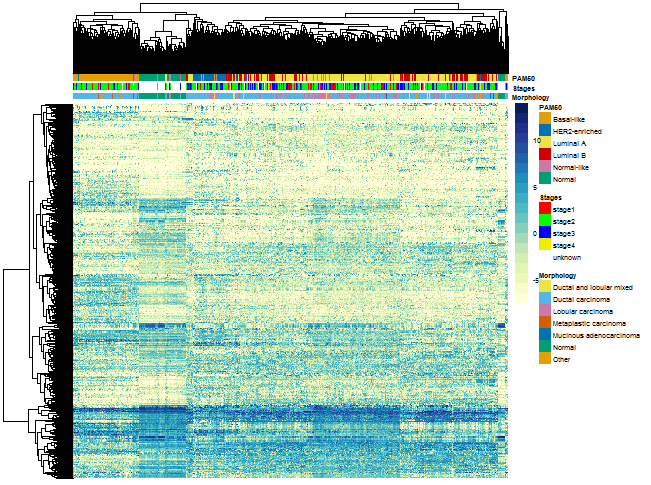
\includegraphics[scale=0.8]{heatmap_top1k.png}
            \caption{Heatmap with clustering on top 1000 highest variance genes (calculated on cancer samples only). The data is clustered by columns (samples) and rows (genes), with dendograms showing how clusters are formed. The colour bars above the heatmap (PAM50, stages, morphology) show the subgroups to which each sample belongs, colour-coded according to the legend on the right. The colours of heatmap represent gene expression intensity according to the scale (high expression - dark blue, low expression - light yellow). The data was clustered with Euclidean distance and average linkage. }
            \label{fig:heatmap1k}
            \end{figure}
    
    First and foremost, the unsupervised clustering was able to form two main clusters: Luminal and non-Luminal samples. Cluster on the right contains the majority of Luminal A and Luminal B samples according to the top colour bar (PAM50). The left hand side cluster contains Basal-like, HER2-enriched, and normal samples. Normal-like subtype is scattered across the entire dendogram, with more notable appearance inbetween Luminal A and normal samples, as expected. The Basal-like cluster is well-defined, which highlights this subtype difference from the rest. The Luminal types are mixed as anticipated. Overall, clustering is in line with the PCA results for PAM50 subtypes. \\
    With regards to stages and morphology colour bars, it can be observed that clustering, much like PCA, was not able to find any distinct major patterns among their subgroups. Again, the sizes of the subgroups may partially be responsible for that. It is a challenge to spot the minority-sized subgroups on the colour bar, and very clear to see how Ductal carcinoma dominates the dataset (light blue, third bar). The colour bar of stages also shows no distinct patterns. 
    
    \newpage
    However, another idea worth investigation is to test how data will cluster if sub-subgroups averages are taken. As stages of cancer progression are of high interest in this project, the averages of each PAM50 subtype at each stage were taken and clustered. Figure \ref{fig:dendogram} shows the resulting dendogram. 
    
        % dendogram
            \begin{figure}[!h]
            \centering
            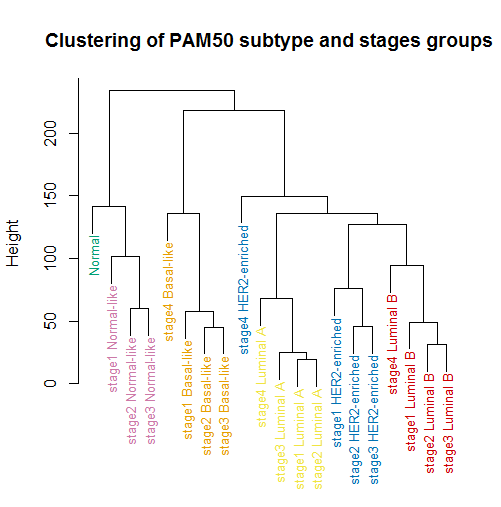
\includegraphics[scale=0.45]{dendogram2.png}
            \caption{Dendogram showing clustering of PAM50 subtypes within stages (averages per stage per subtypes)}
            \label{fig:dendogram}
            \end{figure}
    
    Remarkably, all subtypes form distinct branch clusters (expect HER2-enriched). Normal and Normal-like samples are the outgroup, understandably, and then Basal-like subtype is also an outgroup to the rest of samples. Luminal types and HER2-enriched are separated to well-defined branches. It is important to note that each subtype cluster has stage 4 branch as an outgroup, with the exception of HER2-enriched stage4, which is only made up of 2 samples perhaps leading to an unstable average. Seeing stage 4 as an outgroup is an important observation, as it is the most different and severe (due to metastasis) stage of cancer progression. \\
    
    Lastly, seeing the samples cluster primarily by PAM50 and only then by stage in Figure \ref{fig:dendogram}, is yet another evidence to what was observed with PCA and heatmap clustering. PAM50 is the main classification effect of breast cancer samples. When using other classification methods, PAM50 subtypes have to be taken into account. For example, comparing two morphologies might now produce expected results if their PAM50 subtype sample composition will be the main driving effect of differences. So the heterogeneity of groups has to be taken into account, and the downstream analysis has to be done on sub-subgroups.  
    
     

    
 
    
    \newpage
    \subsection{Cofactors and batch effects}
    
    Morphology, cancer stages, and PAM50 molecular subtype are the expected main sources of variation in the dataset, namely biological variation. However, in a large and heterogeneous dataset such as TCGA-BRCA there are potentially several other sources of variation that may be contributing to the differences in gene expression between samples. Having sufficient clinical and meta annotation for the present samples allows us to explore potential sources of technical variation.
    %AGE is a standard covariate
    Among the available annotations, the most interesting ones are the patient age group, year sample was taken, and tissue source site. These were explored with PCA to visualise any outlying subgroups that may be creating an unwanted batch effect.
    Exploring the samples by year may identify significant differences between years, as the lab protocols for sample processing would have changes in the given years (1988-2013). Such differences could also be observed between the source sites, i.e. clinical institutions and research centers where the original samples were handled. 

    One-dimensional PCA plots were used to visualise variation over the years and across the sample sites. As there are many (>20) subgroups in both year ans site data, PCA scatter plots are not helpful for spotting outlying subgroups. 
    
    Figure \ref{fig:1dpcayear} shows the first 6 PCs of PCA of the year data. Each boxplot represents samples taken in a single year, with individual years shown as gitter-dots to visualise each year group approximate size and sample variation within it (according to y-axis). The boxplots are shown for years in sequential order (1988-2013). 
        
            % 1D PCA YEAR
            \begin{figure}[!h]
            \centering
            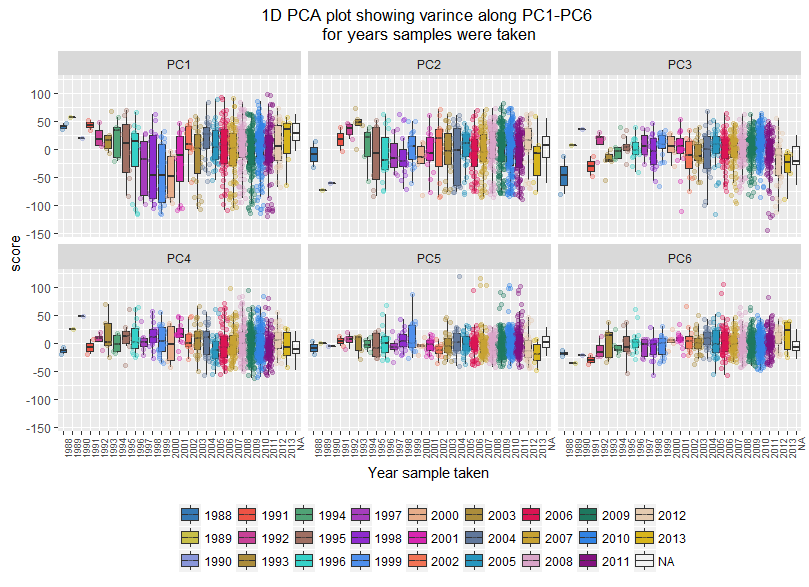
\includegraphics[scale=0.45]{1dpcayear.png}
            \caption{One-dimensional PCA plots showing variance along PC1-PC6 for all samples (cancer and normal) taken in years 1988-2013. The points over each box plot represent samples and their variation on the y-axis scale, to give a better indication of year group size and sample variation within it}
            \label{fig:1dpcayear}
            \end{figure}
    
    
    Overall, it is evident that there is a lot of variation between the years. This is especially the case for the earlier years, however, this is partially due to low number of samples taken in those years.  The variation stabilises after year 2005, which can be explained by the fact that this is when the pilot of TCGA project started and the universal protocols were introduced. Also it is can be seen that the majority of samples were collected after that time point. An observation worth noticing is that samples in years 1997-2000 appear to be quite different to previous and following years (PC1). This could have had a very serious batch effect on the downstream analyses, and had to be explored further.\\
    
    As established in the previous section, we expect PAM50 subtypes to be the main point of interest for further investigation, therefore, it was crucial to check the sample composition of every year group in terms of PAM50 subtypes to make sure that, for example, a particular subtype was *not*  collected in only one year, which would be confounding the dataset exploration in that context. Figure \ref{fig:baryear} shows the stacked barplot of all samples organised by year.  Each bar shows the total count of samples in a year, and the proportion of samples of each PAM50 subtype are coloured according to the legend. 
    
    
             % bar per year
            \begin{figure}[!h]
            \centering
            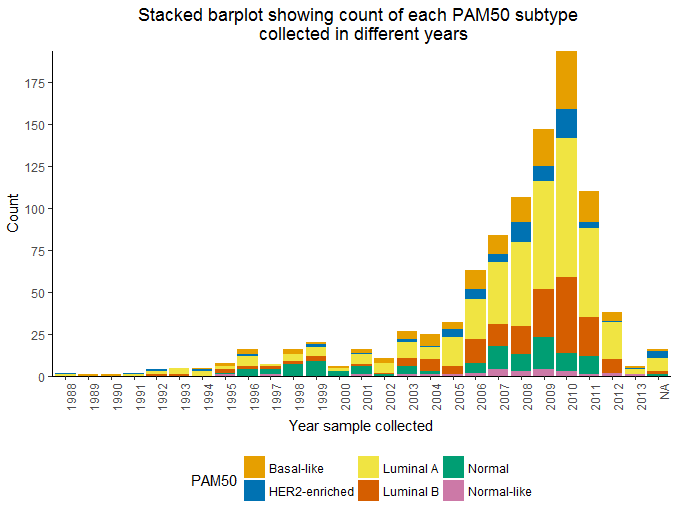
\includegraphics[scale=0.7]{bar_year.png}
            \caption{Stacked barplots of sample counts per year (1988-2013). The coloured proportions represent PAM50 subtypes samples within each year group. }
            \label{fig:baryear}
            \end{figure}
    
    As already noted from 1D PCA plot fro year data, the total number of samples in the earlier years is marginally smaller than in the last decade of given years. Overall, the distribution of PAM50 subtypes in each year is well-balanced,  although some years inevitably have no normal samples and/or samples of a specific subtype. On the whole, the dataset is not confounded by a particular year-subtype combination.  Moreover, visualising data in this way has shed light on the abnormality in years 1997-2000 seen in 1D PCA plot. It can be seen in Figure \ref{fig:baryear} that these years have about 50\% composition of normal samples in them, which is not the case for all other years. Having such high proportion of normal samples in them, makes their mean seem different. Appendix \ref{} shows a 1D PCA plot for cancer samples only, confirming this possible explanation, i.e. years 1997-2000 do not stand out from the rest if only cancer samples are included in the analysis. \\
    
        %sites
    \newpage
    As with year data, the sample source data also had to be explored and variation among sources assessed. Figure \ref{fig:1dpcatss} shows a 1D PCA plot analogous to the one showing variation for samples grouped by year. This plot shows variation for all samples grouped by samples source site (24 sites in total).\\  
            
            % 1D PCA YEAR
            \begin{figure}[!h]
            \centering
            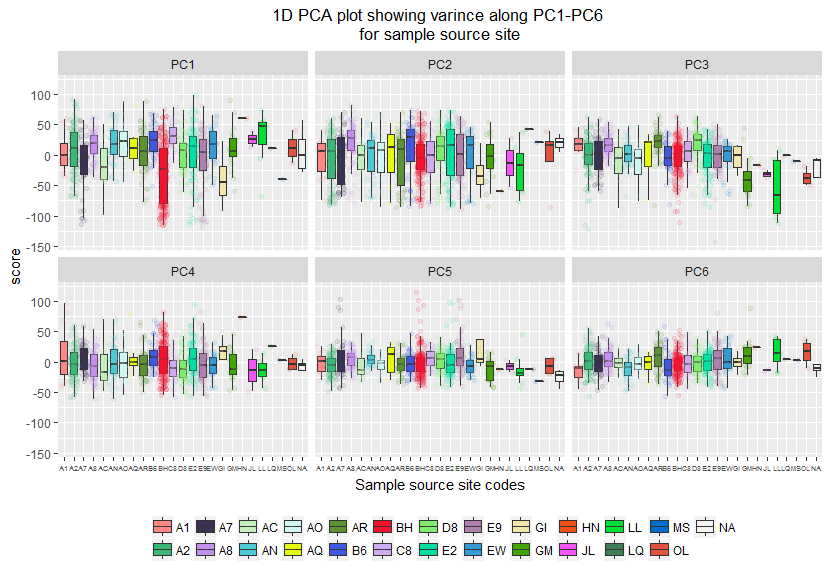
\includegraphics[scale=0.45]{1dpcatss.png}
            \caption{One-dimensional PCA plots showing variance along PC1-PC6 for all samples (cancer and normal) from different source sites (two letter abbreviations; NA - site unknown). The points over each box plot represent samples and their variation on the y-axis scale, to give a better indication of year group size and sample variation within it}
            \label{fig:1dpcatss}
            \end{figure}

    It is clear that the variation between source sites exists, as anticipated. As with year data, some source groups have very few samples, which makes the variation between them and large groups more prominent. One source site that really stands out (PC1) is BH (red). A possible explanation to this could have been that the sample handling protocol at this site is very different  from the rest, or, as it turned out, this differences has the same cause as the difference seen in year data.\\
    
              % bar per tss
            \begin{figure}[!h]
            \centering
            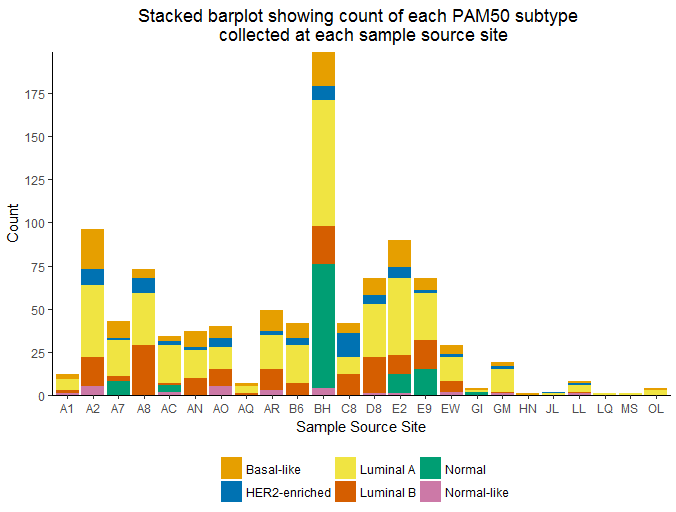
\includegraphics[scale=0.5]{bar_tss.png}
            \caption{Stacked barplots of sample counts per source site (alphabetic order). The coloured proportions represent PAM50 subtypes samples within each year group. }
            \label{fig:bartss}
            \end{figure}
    
    The source site data was visualised as stacked bar plots to inspect sample subtype variety coming from each site, Figure \ref{fig:bartss}. As observed on the 1D PCA plot, some sites have very few samples coming from them. The larger groups are relatively well-balanced in terms of their PAM50 subtype composition, with the exception of Normal-like, which comes only from 7 sites. This is, however, expected, as there are only 26 Normal-like samples in total. Another observation, which may be of bigger concern, is that the majority of normal samples come from one site, BH. This should not affect downstream analyses, as we are interested in differences between cancer subgroups. But seeing this explains the abnormal variation seen in 1D PCA plot for this site. As with year data, this one site is ~50\% composed of normal samples, making it appear very different from the rest as a group. If analysis is done only on cancer samples, this is no longer the case (Appendix \ref{}). 
    
  
    
    

    
    %age groups
    


\section{Looking for Autophagy signatures}

    \subsection{Differential Expression Testing}
    
        \subsubsection{Enrichment Analysis}

    \subsection{Soft clustering}
    
    %identify distinct transcriptome clusters
    %classify genes into groups
    
        \subsubsection{Enrichment Analysis}
    %     The expression profiles of these 348 genes were sorted into 5 clusters by using the fuzzy c-means algorithm implemented in the R package Mfuzz (20). The Mfuzz package uses a “fuzzy” clustering approach to compute the strength of the association of each gene with the central behavior of the cluster, referred to as a “fuzzy score.” The fuzzy scores for each gene sum to 1. This allows one to define a set of genes that associate with each cluster with a high probability, while other genes may not have a high score for association with a single cluster but may instead have scores that allow partial placement in more than one cluster. This approach is more flexible and less sensitive to experimental noise than traditional “hard” clustering, where each gene must belong to one and only one cluster.
 
% Table S1 in the supplemental material shows each of the 348 genes assigned to the 5 clusters and their individual fuzzy scores. The median fuzzy score for each cluster was >0.98, and the average fuzzy score was >0.9, indicating strongly correlated behaviors of the genes within each cluster with respect to changes in growth rate and substrate. Thus, each cluster has a core set of genes with very high fuzzy scores (i.e., close to 1) which indicate that their collective expression behavior is strongly correlated with that of other members of the cluster with respect to their changes in growth rate and substrate. Moreover, the lack of significant overlap of genes between the clusters also supports the unique characteristics of the clusters and their embedded genes.



 
% To overcome the limitations of hard clustering, soft clustering can be applied o
% ering several advantages to researchers [1, 2]. First, it generates accessible internal cluster structures, i.e. it indicates how well corresponding clusters represent genes/proteins. This additional information can be used for a rened search for regulatory elements. Second, the overall relation between clusters, and thus a global clustering structure, can be dened. Additionally, soft clustering is more noise robust and a priori pre-ltering of genes can be avoided. This prevents the exclusion of biologically relevant genes/proteins from the data analysis.



\section{Downstream}


\chapter{Discussion}
%Understanding of autophagy role in cancer is becoming an increasingly intriguing area of research as the two constituting fields -- breast cancer and autophagy -- have seen a lot of progress individually in the recent decade. This project aimed to identify the expression signatures of autophagy-related genes in the breast cancer transcriptomics data available from TCGA. 

Through rigorous exploratory analysis the dataset was extensively investigated and the main patterns characterising the available samples established. The three main classification methods  used to stratify the samples were: cancer stage, tumour morphology, and PAM50 intrinsic molecular subtype. Thus, the hypothesis-driven analysis aimed to identify a subset of samples described by one of the classification methods, whose expression has a notable autophagy enrichment. To identify autophagy expression signatures, two complementary analysis methods were used -- differential expression testing and soft-clustering. 

In DE analysis, a multitude of DE tests were performed to explore all possible combinations of samples defined by different classification methods, and the identified sets of differentially expressed genes were tested for autophagy enrichment. Soft-clustering aimed to detect clusters of genes that have similar collective expression behavior that is strongly correlated with that of other members of the cluster with respect to their changes across cancer progression stages. Soft-clustering was performed on separate cancer subtypes, then, enrichment analysis was used to identify expression patterns where autophagy genes are overrepresented. Following that, a comparative analysis of the results produced by the two methods helped to identify a set of autophagy genes that could be used as a starting point for further exploration of autophagy role in cancer.

Exploratory analysis of TCGA-BRCA dataset was a crucial part of this project. Firstly, it has confirmed the view that is now widely accepted in the breast cancer research community on the extreme heterogeneity of this disease, and the fact that the cancer patients can most accurately be classified into prognostic groups by their intrinsic molecular profile rather than by tumour morphology and stage. The major differences between PAM50 subtypes were highlighted by PCA, hierarchical clustering, as well as differential expression testing, where individuals subtypes had considerably more DEGs among each other than tumour morphologies or stages. 

In fact, neither exploratory analysis nor differential expression testing have found any strong differences between morphological groups or stages. The PCA plots for both did not reveal any PCs that describe the proposed sample subgroups sufficiently well. DE analysis found exceptionally low number of DEGs between cancer stages (even stage 1 and stage 4), and also not a great amount of DEGs between two major established morphologies, Lobular and Ductal carcinomas. This result was surprising, but the explanation was proposed to be in the underlying imbalanced composition of the subgroups being compared.

In the exploratory analysis it was shown how disproportionate the comparison subgroups are both in terms of their sample size and PAM50 composition. PAM50 composition of subgroups is important as it explains the main driving force that defines variation between samples. This has got two implications. First, if the groups are too mixed/heterogeneous (i.e. made up of various PAM50 subtypes), then it is difficult to capture differences between them, as the variation signal is too mixed and thereby weak. Second, if two groups that are being compared are exclusively made up of two different PAM50 subtypes, then the difference between them is likely to be driven by PAM50. A clear example of this was found when comparing Mucinous and Metaplastic morphologies, which are exclusively made up of Luminal and Basal samples, respectively. These two morphologies were found to have the largest number of DEGs between them compared to morphologies, in addition to being very clearly separated by PCA. However,  the true source of their variation is difficult to define. 

To tackle the problem of heterogeneity created by the strong influence of PAM50 profiles on other classifications, DEA with combined models was performed. It allowed to characterise differential expression between individual stages or morphologies within each PAM50 subtype. In this way, for instance, differentially expressed genes between Lobular and Ductal carcinomas within each PAM50 subtype were identified. 

However, enrichment analysis results were ambiguous and largely unsuccessful in identifying autophagy signatures in any specific subgroups of samples. The main reocurring observed trend was that autophagy-related genes are enriched among groups of downregulated genes in various cancer subgroups (including individual morphologies and stages). Interestingly, there was no enriched autophagy signature between different stages of cancer, which is something that is often brought up in the literature describing the behaviour of autophagy processes in cancer. Moreover, the PAM50 subtypes, between  which  large numbers of DEGs were identified, had no significant autophagy signatures in any of the tested contrasts. Therefore, it was concluded that the main observed and quantified autophagy signature in this breast cancer dataset is the overall downregulation of autophagy-related genes in cancer versus normal, regardless of stage or subgroup.

In line with that, soft-clustering analsyis results have shown that the marority of autophagy genes are assigned to the cluster representing downregulation at all stages expression pattern, and which was consistently found to be significantly enriched for autophagy in different subtypes, either at  all genes or transcription factors-only level. 

Considering the agreement between the results of the two methods on the putative signature of autophagy genes in the downregulation trend, comparative analysis was performed. For each PAM50 subtype, a list of candidate genes that exhibit complete downregulation in cancer (i.e. downregulated at all stages vs normal) was produced. Hence, the direction from here is to seek collaboration with the experts in the autophagy fields to guide a more informed biological interpretation of the potential role and the impact of downregulation of the identified genes. 

Overall, it is important to highight the significance of finding the downregulation in cancer trend to be the autophagy signature in this dataset. In broad sense, it makes sense to see a subset of  autophagy-related genes to be downregulated in cancer. Deregulated autophagy means that the basal turnover of damaged molecules is impaired, which has an oncogenic impact. Furthermore, seeing autophagy genes downregulated consistently at all stages but compaed to normal, gives an indication of the part of the mechnism twhse inactivation is cancer-related in general. So here we have ‘natural’ autophagy inhibition signature.

However, the literature on autophagy role in cancer often brings up the ‘dual role’, which involves upregulation of  autophagy at different stages of cancer progression with opposite consequnces. The results of this project did not show any statistically significant indication of autophagy genes being upregulated at any specific stages or cancer in general. Although among the soft-clustering results there were several clusters of genes with potentially interesting expression patterns in relation to stage-specific upregulation,  the enrichment analysis did not indicate hat those clusters have signisicant autophagy signature.


The inability to identify any autophagy signatures being upregulated at significant (or significant at non-adjusted p-value level, as p-value cut-off are arbitrary) level, also bring the discussion of the potential limitations of this study. Firstly, it has to be reiterated that imbalanced subgroups sized are very likely to be contribution to results both of EDA and analyses looking for groups of genes to test for enrichment. As brought up previously, the number of samples in stage 4 in this analysis setup makes all the compatisons involving it questionable. It also is impossible to make stage wise comparison of morphological groups as all samples belong to morphology. Also the comparisons within individual PAM5 subtypes, both in DEA and clustering is a bit unreliable, as for example, expression of Basal-like and HER2-enriched samples of stage 4 is characterised by only two samples each (see Table 3.1). Hence, … Perhaps, expectig to see a change in expression at the later stages of cancer progression with the available data was too ambitons, due to the fact that the most prominent literature-acknowledged   However, seeing that pattern in the results is interesting indeed as this is the stage where some crazy changes start happening and this is is where upregulatin of autophagy may have an oncogenic role. However, it is still a primary tumour samples, and for true assessment of autophagy genes expression pattern in metastasis we need metastasis samples.  

Furthermore, one important aspect that was not taken into account in this project is the information on treatments each patient has received. This information was not readily available at the times where it could have been utilised to benefit this project , but now we think that perhaps we see autophagy downregulated as a consequence of treatment that were supposed to inhibit autophagy. 




\section{Future directions}

%5. Discuss the implications of your study for future research and be specific about the next logical steps for future researchers.


The first main direction of this project is to start an active collaboration with the autophagy experts at DCRC by making the identified list of candidate genes available to them. Then it will have to discussed and decided which hits could sent for experimental validation in MCF7 breast cancer cell lines. 
Then also the observed other trends such as interesting cluster patterns in specific subtypes should also be analysed with more autophagy knowledge. 

As the main constraint that is thought to have the negative effect on identifying signature in a specific breast cancer subtype or stage is the lack of samples in the groups, it is perhaps a good idea to explore other cohort of samples with the same analysis setu to see if the results are reproducible  TCGA is of course the  a rich source of data., but 

Smaller groups but better balanced could give more answers 


it is not a difference that we can see just using data at the transcriptional levels (it could be regulation of protein levels, ptms, cancer mutations etc) stimulating directions for people that will arrive after you.


It could be that in this specific case breast cancer we do not observe it but in other cancer studies or cohort we might find it considering the tremedous heterogeneity of cancer mechanisms even within the same subtype. It can be that there is no enrichment with the methods that we are using but that some of the autophagy genes are in any case playing a role because they get up and down regulated  and cross-talk with other pathways or that our list unfortunately still doesn't cover the complicate spectrum of autophagy-related genes

I will discuss how the hypothesis has been demonstrated by the new research and then show how the field's knowledge has been changed by the addition of this new data

-- discussion starts with the interpretation of the results, then moves outwards to contextualize these findings in the general field.




\section{Conclusion}
%4. State the major conclusions from your study and present the theoretical and practical implications of your study.




\cleardoublepage
\addcontentsline{toc}{part}{\small Acknowledgements}
\addtocontents{toc}{\protect\vspace{-1.5em}}
\chapter*{Acknowledgements}
\blindtext
% I would like to thank the Computational Biology Laboratory at the Danish Cancer Research Centre for
% allowing me to join their group to conduct a university research project.
% I am especially thankful to Dr Elena Papaleo for her professional guidance and valuable support throughout
% the project. Her ability to explain difficult bioinformatics concepts and show how to correctly use the software
% to answer structural biology questions has been greatly appreciated and has enabled me to complete high
% quality work.
% I would also like to thank the other members of the group, including Matteo Tiberti, Matteo Lambrughi and
% Thilde Terkelsen for advice throughout the project.

\cleardoublepage
\addcontentsline{toc}{part}{\small Bibliography}
\addtocontents{toc}{\protect\vspace{-0.2em}}
\printbibliography

\backmatter
\end{document}
